\emph{Como producto del trabajo presentado en este capítulo surgieron los artículos de congreso titulados ``UNSL at eRisk 2019: a Unified Approach for Anorexia, Self-harm and Depression Detection in Social Media''\footnote{\url{http://ceur-ws.org/Vol-2380/} (Sección ``eRisk - Early Risk Prediction on the Internet'').} y ``Towards Measuring the Severity of Depression in Social Media via Text Classification''.\footnote{\url{http://sedici.unlp.edu.ar/bitstream/handle/10915/91042/Documento_completo.pdf?sequence=1}}}

\

En capítulos anteriores se introdujeron el modelo propuesto y una extensión del mismo, denominada $\tau$-SS3. La evaluación de estos modelos se llevó a cabo utilizando los datos disponibles de las ediciones 2017 y 2018 del eRisk para distintas tareas de detección anticipada de riesgos.
El presente capítulo describe nuestra participación en la edición 2019 del eRisk y tiene como objetivo principal la evaluación de la robustez y el desempeño de los modelos propuestos, utilizando nuevas medidas de desempeño no consideradas anteriormente y dos nuevos conjuntos de datos.
Además, al tratarse de una participación, este capítulo también permite verificar en qué medida los resultados obtenidos, al poner a prueba el modelo en la práctica, son efectivamente consistentes con los obtenidos en los capítulos anteriores por medio de la experimentación controlada.

% El eRisk 2019 contó con dos tareas de detección anticipada de riesgos, respectivamente, una tarea de detección anticipada de anorexia y otra de conductas autodestructivas.
% Afortunadamente, los resultados conseguidos en estas tareas reforzaron aquellos obtenidos en los capítulos anteriores, mostrando que SS3 podría llegar a ser un clasificador robusto y eficiente para lidiar con tareas de este tipo, ya que, de entre todos los modelos y para ambas tareas, fue el más rápido en procesar los datos y el que obtuvo los mejores valores $ERDE_5$ y $ERDE_{50}$, el mejor desempeño promedio en las medidas basadas en ranking y, además, obtuvo los mejores valores de $precision$ y $F1$ para una de las tareas.
% Finalmente, en la tarea T3 obtuvo los mejores valores de AHR y ACR, y el segundo mejor ADODL y DCHR.
% Esto fue bastante notable teniendo en cuenta que aquí se usó el mismo clasificador para completar los cuestionarios BDI de los usuarios, que es una tarea completamente diferente de las otras dos tareas binarias ``sí o no''.
% SS3 was the fastest method and obtained the best $ERDE$ and overall best ranking-based measures in all the tasks.
% Additionally, it obtained the best $Precision$, $F1$ and $F_{latency}$ for task T2.
% Finally, in task T3, it obtained the best AHR and ACR values, and the second-best ADODL and DCHR.
% This was quite remarkable taking into account that the same classifier was used here to fill users' BDI questionnaires, which is a task completely different from the other two ``yes or no'' tasks.


% \section{Introducción}%Introduction

%This year we decided not to use other models other than SS3 because of the change in the way data was released, i.e. a more realistic item-by-item release of data. The other models we used last year based on TVT\cite{errecalde2017} were no longer applicable since they were designed to work with chunks and not text streams. 

%Additionally, this year we decided to put the robustness of SS3 into the test by using the same hyper-parameter configuration in all the 15 runs for the 3 tasks (T1, T2, and T3). Thus, the hyper-parameters values were set to $\lambda =\rho=1$ and $\sigma= 0.455$, which were the same values used in \cite{burdisso2019}, and for which SS3 has shown to be quite robust in terms of ERDE performance measure.


\section{Introducción}

Como se describe más detalladamente en el reporte general del eRisk 2019 \cite{losadaetal2019}, esta edición se organizó de manera similar a la de los años anteriores ya que cada grupo de investigación tuvo permitido participar con un máximo de hasta 5 modelos y el conjunto de datos de cada tarea se construyó utilizando usuarios de Reddit.
Sin embargo, hubo cambios en la forma de llevar a cabo la fase de prueba de los modelos y se enriqueció la forma de evaluarlos al introducir nuevas medidas de desempeño.

Más en detalle, en esta edición, finalmente se cambió la forma en la que las publicaciones de los usuarios se entregan a los modelos durante la fase de prueba, dejándose de lado el uso de bloques de publicaciones y utilizándose, en su lugar, el mismo enfoque utilizado en el \autoref{cap:ss3} para el segundo escenario de experimentación, más realista (\autoref{subsec:exp-scenario2}), en donde los usuarios fueron procesados una publicación a la vez.
Para llevar esto a cabo, se configuró un servidor encargado de proporcionarle a los modelos participantes el flujo de publicaciones de cada usuario.\footnote{Más información sobre el servidor se puede encontrar en el sitio web del eRisk: \url{http://early.irlab.org/server.html}.}
Así, durante la fase de prueba, los modelos debieron conectarse al servidor tanto para solicitar las publicaciones, de a una por vez, como para enviar la decisión tomada sobre cada usuario luego de recibirlas ---el envío de esta decisión fue obligatorio, de lo contrario no se podía recibir la siguiente publicación del usuario. En particular, luego de leer cada publicación, los modelos debían responderle al servidor con un $1$ o un $0$ para indicar, respectivamente, que el usuario estaba en riesgo o que aún era necesario procesar más publicaciones para poder decidirlo ---de esta manera, cada modelo fue libre de detenerse y realizar la alerta temprana en cualquier punto de la cronología de los usuarios.

Una vez terminada la fase de prueba, se evaluó el desempeño de todos los modelos y se publicaron los resultados obtenidos por todos los participantes. Como se detallará en la siguiente sección, en esta edición del eRisk, los modelos fueron evaluados utilizando, además de la medida $ERDE$, nuevas medidas de desempeño que capturan distintos aspectos vinculados tanto a la clasificación anticipada como a la estimación del nivel de riesgo de los usuarios.
% En 2019, el laboratorio tenía tres tareas de estilo de campaña. Dos de ellos tenían la misma orientación de tareas anteriores de eRisk pero cambiamos la forma en que se publicaban los datos y, además, ampliamos el conjunto de medidas de evaluación.
% Estas dos tareas estaban orientadas a la detección temprana de signos de anorexia y autodestructivas, respectivamente.
% La tercera tarea, que era completamente nueva, estaba orientada a analizar el historial de publicaciones de un usuario y extraer evidencia útil para estimar el nivel de depresión del usuario.
% Más específicamente, los participantes tenían que procesar las publicaciones del usuario y, a continuación, estimar las respuestas del usuario a un cuestionario de depresión estándar. Estas tres tareas se describen en las siguientes secciones de este documento general.




\section{Medidas de Desempeño}

En esta sección se describen brevemente las medidas de evaluación utilizadas para medir el desempeño de los modelos participantes en esta edición del eRisk. 
En particular, además de reportarse el tiempo que le tomó a cada equipo completar cada tarea, se utilizaron dos tipos distintos de medidas, las centradas en la decisión y las basadas en ranking, las cuales se describen en las siguientes dos subsecciones.



\subsection{Medidas Centradas en la Decisión}
\label{sec:medidas_decision}

Esta forma de evaluación gira en torno a las decisiones que los modelos deben tomar para cada usuario.
En este grupo se encuentra la medida $ERDE_o$ que se ha venido utilizando tanto en este trabajo como en las ediciones anteriores del eRisk.
Sin embargo, en esta edición 2019 del eRisk también se incorporó una nueva medida, denominada como $F_{latency}$ \cite{sadeque2018measuring}, la cual, al igual que $ERDE_o$, fue diseñada para combinar tanto la efectividad de la clasificación como su demora.
El calculo de esta nueva medida se basa en multiplicar la medida tradicional $F_1$ por un factor de penalización basado en la mediana de la demora de todas las decisiones.
Más específicamente, a cada decisión \emph{correcta} de emitir un alerta para un usuario $u$, luego de haber leído $k_u$ publicaciones, se le asigna la siguiente penalización:

$$penalty(k_u) = -1 + \frac{2}{1 + exp^{-p(k_u - 1)}}$$

donde $p$ es un parámetro que permite determinar qué tan rápido debe aumentar la penalización.
En particular, para las tareas del eRisk se estableció un valor de $p$ tal que la penalización sea igual a $0.5$ en la mediana del número de publicaciones de los usuarios.
Esta ecuación produce que la penalización comience siendo $0$, cuando la decisión se toma luego de leer la primer publicación (\emph{i.e.} $penalty(1) = 0$), pero luego vaya aumentando paulatinamente conforme se necesitan leer más publicaciones, como se muestra en la \autoref{fig:penalty}.
%no entiendo bien esta oracion
%
%
%
%
%
%
\begin{figure}[t]
    \centering
    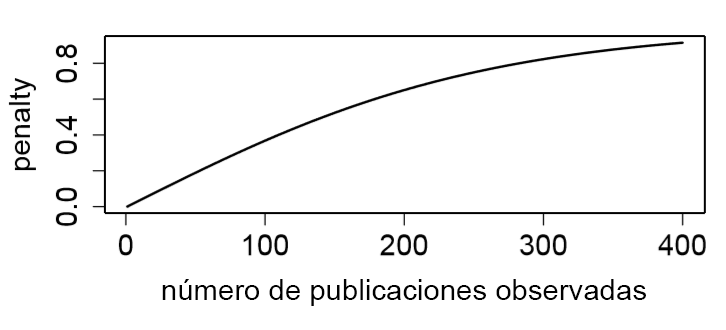
\includegraphics[width=.6\textwidth]{images/penalty}
    \caption{Aumento de la penalización $penalty(k_u)$ en relación al número de publicaciones observadas ($k_u$) antes de tomar la decisión.}
    \label{fig:penalty}
\end{figure}

Más precisamente, la medida $F_{latency}$ se calcula multiplicando la medida $F_1$ tradicional con un valor que representa la velocidad con la que se clasificaron todos los usuarios del conjunto de prueba.
Este último valor se denomina $speed$ y su cálculo se realiza utilizando la mediana de todas las penalizaciones $penalty(k_u)$ obtenida para todos los usuarios, $u$, del conjunto de prueba. En símbolos, siendo $U_{vp}$ el conjunto de usuarios del conjunto de prueba clasificados correctamente como en riesgo (verdaderos positivos), $speed$ se define como:

$$speed = 1 - \text{mediana}\{penalty(k_u) / u \in U_{vp}\}$$
% $$speed = (1 - \text{median}\{penalty(k_u) / u \in U, d_u = g_u = 1\})$$

Y finalmente, $F_{latency}$ se define como:

\begin{equation}
F_{latency} = F_1 \times speed
\label{eq:flatency}
\end{equation}


\


La medida $F_{latency}$ surge como una alternativa a la medida $ERDE_o$ que intenta solucionar algunos defectos de esta última~\cite{sadeque2018measuring}.
Por ejemplo, si bien la medida $ERDE_o$ permite realizar comparaciones relativas entre modelos,\footnote{Ya que por definición se tiene que mientras más rápido y efectivo sea un modelo, más cercano a $0$ será su valor $ERDE_o$, es decir, más cercano a nulo será el error acumulado.} su semántica en término de su valor absoluto no es tan clara.\footnote{¿Qué significa que el valor $ERDE_5$ obtenido haya sido de, por ejemplo, $11.31\%$?¿fue el modelo rápido o lento?}
En su lugar, la medida $F_{latency}$ posee una semántica más clara debido a que su valor se apoya en la medida $F_1$ tradicional, cuya semántica es bien conocida y captura la efectividad de la clasificación, y un valor de penalización que explícitamente captura la demora de la misma.
Además, en la medida $ERDE_o$, la penalización por la demora en la clasificación es virtualmente binaria, es decir, será siempre $0$ para modelos clasificando correctamente a los usuarios antes de procesar $o$ publicaciones, y $1$ para un número mayor de publicaciones. 
En su lugar, la penalización en la medida $F_{latency}$ va aumentando gradualmente conforme se procesen más documentos.
Sin embargo, creemos adecuado no pensar la medida $F_{latency}$ como superior a $ERDE_o$, sino más bien como capturando distintos aspectos de la clasificación anticipada, es decir, al igual que las medidas tradicionales $recall$ y $precision$ no son superiores la una de la otra, sino que ambas capturan distintos aspectos de la clasificación de documentos, $ERDE_o$ y $F_{latency}$ nos brindan información vinculada a distintos aspectos de la clasificación anticipada.
Por ejemplo, debido a que la medida $F_{latency}$ utiliza la medida $F_1$, su utilización resaltará a modelos que le asignen la misma importancia tanto a $recall$ como a $precision$, mientras que la medida $ERDE_o$ resaltará a los modelos que prioricen $recall$ por sobre $precision$,\footnote{Esto se debe a la forma en que se calcula la medida $ERDE_o$ (\autoref{eq:erde}), siendo el costo de los falsos positivos ($cfp$) considerablemente más pequeño que el de los falsos negativos ($cfn$).} lo que no es necesariamente malo teniendo en cuenta que se lidia con tareas de riesgo en donde cada usuario (positivo) no detectado es una vida en riesgo.
De la misma manera, el hecho de que la penalización de la medida $ERDE_o$ sea binaria no necesariamente representa un defecto si se tiene en cuenta la naturaleza binaria de cualquier tarea de riesgo, en donde existe un punto específico en el tiempo que se intenta anticipar y que, pasado el mismo, ya es demasiado tarde para una clasificación efectiva\footnote{Tal vez una mejor manera, más realista, de utilizar la medida $ERDE_o$ podría obtenerse simplemente al asignar, en lugar de un único valor $o$ fijo para todos los usuarios en riesgo, un valor $o$ específico para cada uno de ellos que refleje el punto en el tiempo al que los modelos deben anticiparse específicamente para ese usuario.} ---a diferencia de otras tareas de clasificación anticipada en las que el costo a pagar por una demora aumenta gradualmente con el tiempo.

% Tenga en cuenta que la mayoría de los valores ERDE están relativamente cerca entre sí, esto se debe a la forma en que se calculó $ERDE$.\footnote{$cfp = \frac{\#positive\_users}{\#users}$ por lo tanto cada usuario, clasificado erróneamente como falso positivo, agregó un valor de $\frac{cfp}{\#users} = \frac{\#positive\_users}{\#users^2} = \frac{73}{815^2} = 0.0001$ al final/informado $ERDE$ (y 0.001 en caso de falso negativo o verdadero positivo después del umbral de $o$).} Cuanto más grande y desequilibrado sea el conjunto de datos, asintóticamente más planos y más cercanos son los valores de $ERDE$ (como sucedió con esta tarea). Por lo tanto, los decimales importan mucho cuando se trata de la medida de $ERDE$. Por ejemplo, en esta tarea, solo una pequeña diferencia de 0.009 (0.9\%) en $ERDE$ en realidad significa que el 12\% de todos los usuarios anoréxicos o no anoréxicos no fueron clasificados adecuadamente, lo cual es una diferencia significativa.


% This metric try to overcome some limitations of ERDE, namely:

% – the penalty associated to true positives goes quickly to 1. This is due to the functional form of the cost function (sigmoid).
% – a perfect system, which detects the true positive case right after the first round of messages (first chunk), does not get error equal to 0.
% – with a method based on releasing data in a chunk-based way (as it was done in 2017 and 2018) the contribution of each user to the performance evaluation has a large variance (different for users with few writings per chunk vs users with many writings per chunk).
% – ERDE is not interpretable.

% En su lugar, $F_{latency}$ has the following nice properties:
% – smooth grow of penalties.
% – a perfect system gets Flatency = 1 .
% – for each user $u$ the system can opt to stop at any point ku and, therefore, now we do not have the effect of an imbalanced importance of users. ????
% – Flatency is more interpretable than ERDE.

% Sin embargo, no coincidimos con los autores, 



% Sin embargo, cualquiera de estas dos medidas tiene el problema de ... entonces también se incluyeron medidas basadas en ranking que son independientes de la decisón y se centran en ver que tan bien los modelos creen que cada usuario está en riesgo. (algo así)

% Sin embargo, en lugar de tener un modelo que clasifique los usuarios, se podría tener un modelo que le asigne un ``grado de riesgo'' a cada usuario y luego le presente a los expertos un ranking ordenado en por grado de riesgo para que ellos tomen la decisión. Este ranking iría constantemente cambiando con forme se vayan procesando nuevas publicaciones.

\subsection{Medidas Basadas en Ranking}

En esta edición del eRisk, como complemento de las medidas $ERDE$ y $F_{latency}$, también se utilizaron medidas basadas en ranking.
Por este motivo, luego de que los modelos solicitaran la siguiente publicación de cada usuario al servidor, se les pidió a los modelos que le respondieran al servidor, no sólo con la decisión sobre cada usuario, sino también con una puntuación que represente el grado de riesgo de cada usuario, estimado por el modelo hasta ese momento.
Luego, ordenando todos los usuarios según la puntuación asignada por el modelo, se puede obtener un ranking de usuarios dado por el grado de riesgo estimado. %por cada modelo participante.
Como consecuencia, en cada instante de tiempo es posible obtener un ranking de usuarios asociado a cada modelo participante ---\emph{e.g.} un ranking luego de leer la primer publicación, uno luego de leer la segunda, y así sucesivamente.
De esta manera se busca simular un enfoque de reordenamiento continuo de usuarios en base a la incorporación de nueva evidencia, lo que en una aplicación de la vida real permitiría que el ranking actual pueda ser presentado a expertos humanos, en cualquier momento que sea necesario ---dichos expertos serían luego los encargados de tomar las decisiones correspondientes analizando a los usuarios con mayor grado de riesgo estimado, es decir, los primeros usuarios del ranking.

La evaluación del desempeño de los modelos en este tipo de escenarios se puede llevar a cabo simplemente utilizando las medidas de calidad de ranking tradicionales del campo de la \emph{Recuperación de Información}.
De esta forma, al medir la calidad de los distintos rankings estaremos evaluando el desempeño de los distintos modelos en relación a qué tan bien estiman el grado de riesgo de los usuarios.
En particular, las medidas de calidad de ranking utilizadas en esta edición del eRisk fueron las medidas $P@k$ y $NDCG@k$. Más precisamente, se utilizaron las medidas $P@10$, $NDCG@10$ y $NDCG@100$, las cuales fueron reportadas, por cada modelo, para 4 rankings distintos, respectivamente, el ranking obtenido luego de leer $1$, $100$, $500$ y $1000$ publicaciones.

La medida $P@k$ se denomina como ``Precisión a los $k$'', y corresponde al porcentaje de resultados relevantes presentes entre los $k$ primeros del ranking. En el caso del eRisk, los resultados relevantes se corresponderían a los usuarios que efectivamente están en riesgo, por lo que en esta tarea la medida $P@k$ es el porcentaje de usuarios en riesgo presentes entre los $k$ primeros resultados del ranking.

La medida $NDCG@k$ del inglés ``Normalized Discounted Cumulative Gain'', es la versión normalizada de la medida $DCG@k$, la cual se calcula como:

$$DCG@k = \sum_{i=1}^k \frac{rel_i}{log_2\left(i+1\right)}$$

Donde $rel_{i}$ es el grado de relevancia del resultado presente en la posición $i$ del ranking. En el caso del eRisk, el grado de relevancia es binario, siendo $1$ para los usuarios en riesgo y $0$ para los que no. La idea principal detrás de este medida es penalizar a los resultados relevantes en relación a qué tan abajo en el ranking hayan aparecido.
Finalmente, la normalización se lleva a cabo en relación al $DCG@k$ que obtendría el ranking ideal,\footnote{En el caso de las tareas del eRisk, el ranking ideal sería el ranking en donde todos los usuarios en riesgo se encuentran al comienzo del ranking y luego el resto de usuarios.} denotado por $IDCG@k$, en símbolos:

\begin{equation}
NDCG@k = \frac{DCG@k}{IDCG@k}
\end{equation}


\section{Detalles de Implementación}
\label{sec:erisk2019implementacion}

% La implementación se llevó a cabo de forma análoga a los capítulos anteriores ya que, como se mencionó al inicio, el fin principal de nuestra participación fue el de comprobar si los resultados obtenidos en la práctica eran, efectivamente, consistentes con los obtenidos en los capítulos anteriores, por medio de la experimentación.

Como el objetivo principal es evaluar más en detalle la robustez y el desempeño de los modelos propuestos en los capítulos anteriores sobre un nuevo conjunto de datos, se utilizaron los mismos valores de hiperparámetros que en los capítulos anteriores, es decir $\lambda=\rho=1$ y $\sigma= 0.455$. Como se describió en el \autoref{cap:ss3}, estos valores fueron originalmente seleccionados para optimizar la medida $ERDE_{50}$ en la tarea del eRisk 2017 y luego, como se observó en el \autoref{cap:tss3}, también mostraron ser robustos en las tareas del eRisk 2017 y 2018, en donde tanto SS3 como $\tau$-SS3 se desempeñaron consistentemente bien en términos de la medida $ERDE$.
Por el mismo motivo, se utilizó nuevamente la suma de vectores como el \emph{operador de resumen} ($\oplus_j$) para todo nivel $j$ y la misma política de clasificación anticipada que en el capítulo anterior ---es decir, los usuarios se clasificaron como positivo tan pronto como el \emph{valor de confianza} positivo, acumulado hasta ese momento, fuese mayor que el negativo.
% Finalmente, con respecto al preprocesamiento, no se utilizó ningún método especial salvo una simple normalización eliminando los acentos y convirtiendo el texto a minúsculas, al igual que en el capítulo anterior.\footnote{
% Se probaron otros métodos como \emph{stemming} y \emph{lemmatization} utilizando el paquete \emph{Natural Language Toolkit} (NLTK) de Python, pero al contrario de lo que esperábamos inicialmente, el rendimiento del modelo se redujo.}

\begin{figure}[t]
    \begin{subfigure}{0.5\textwidth}
        \centering
        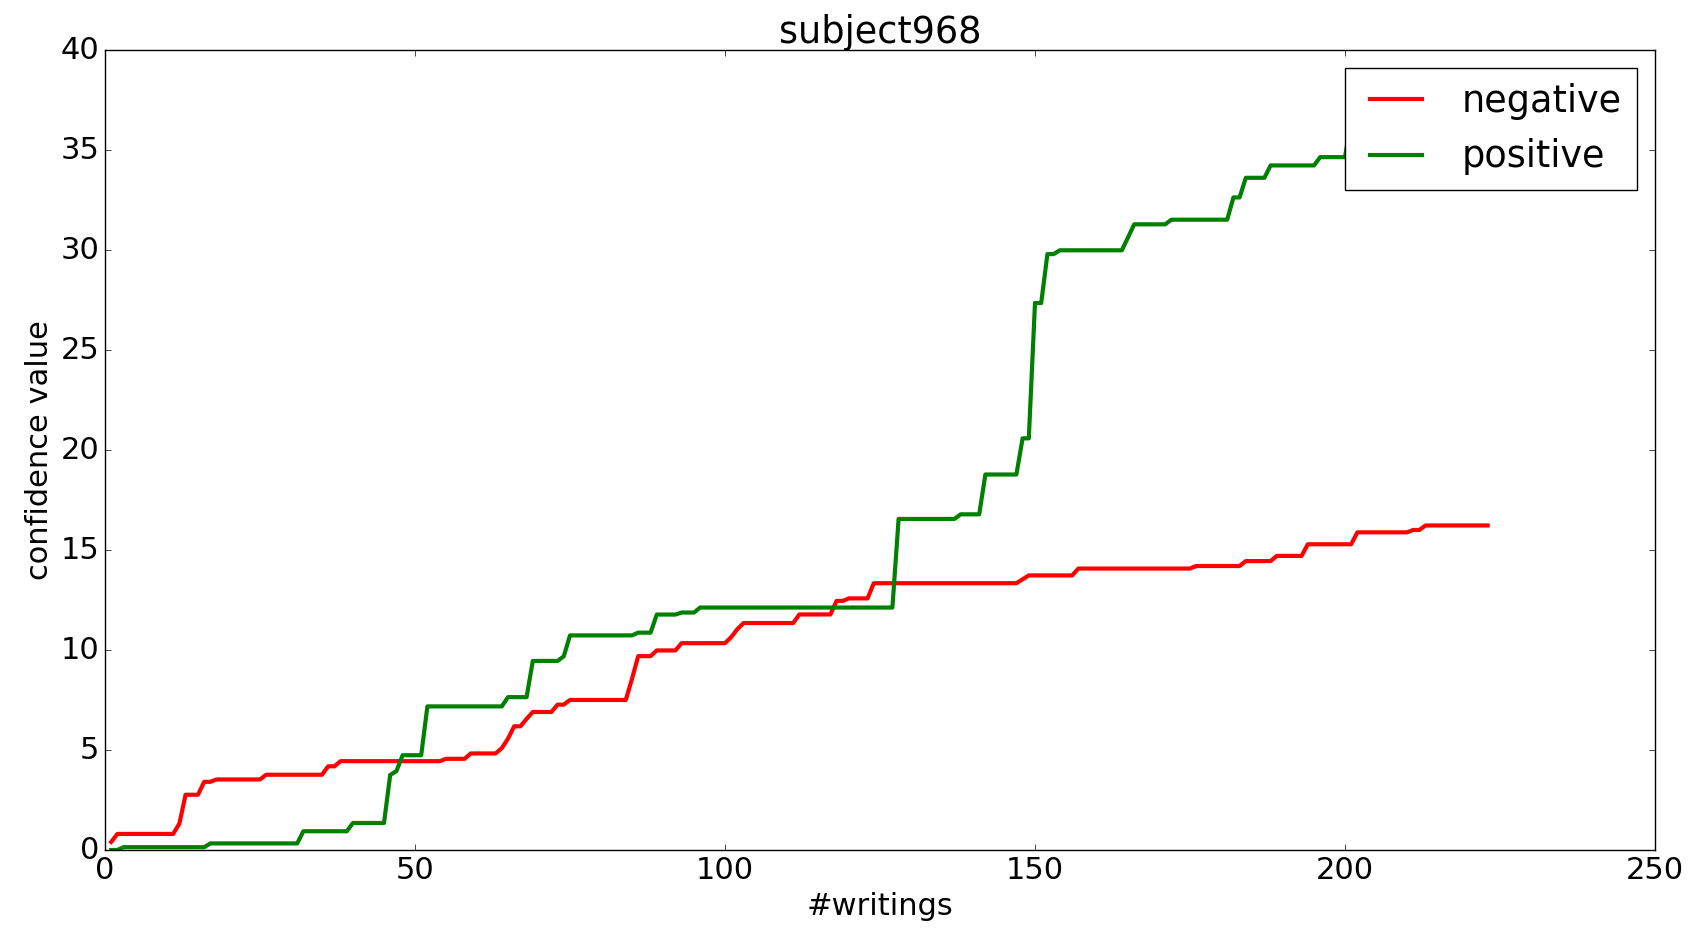
\includegraphics[width=80mm]{images/subject968}
        \caption{}
    \end{subfigure}
    \begin{subfigure}{0.5\textwidth}
        \centering
        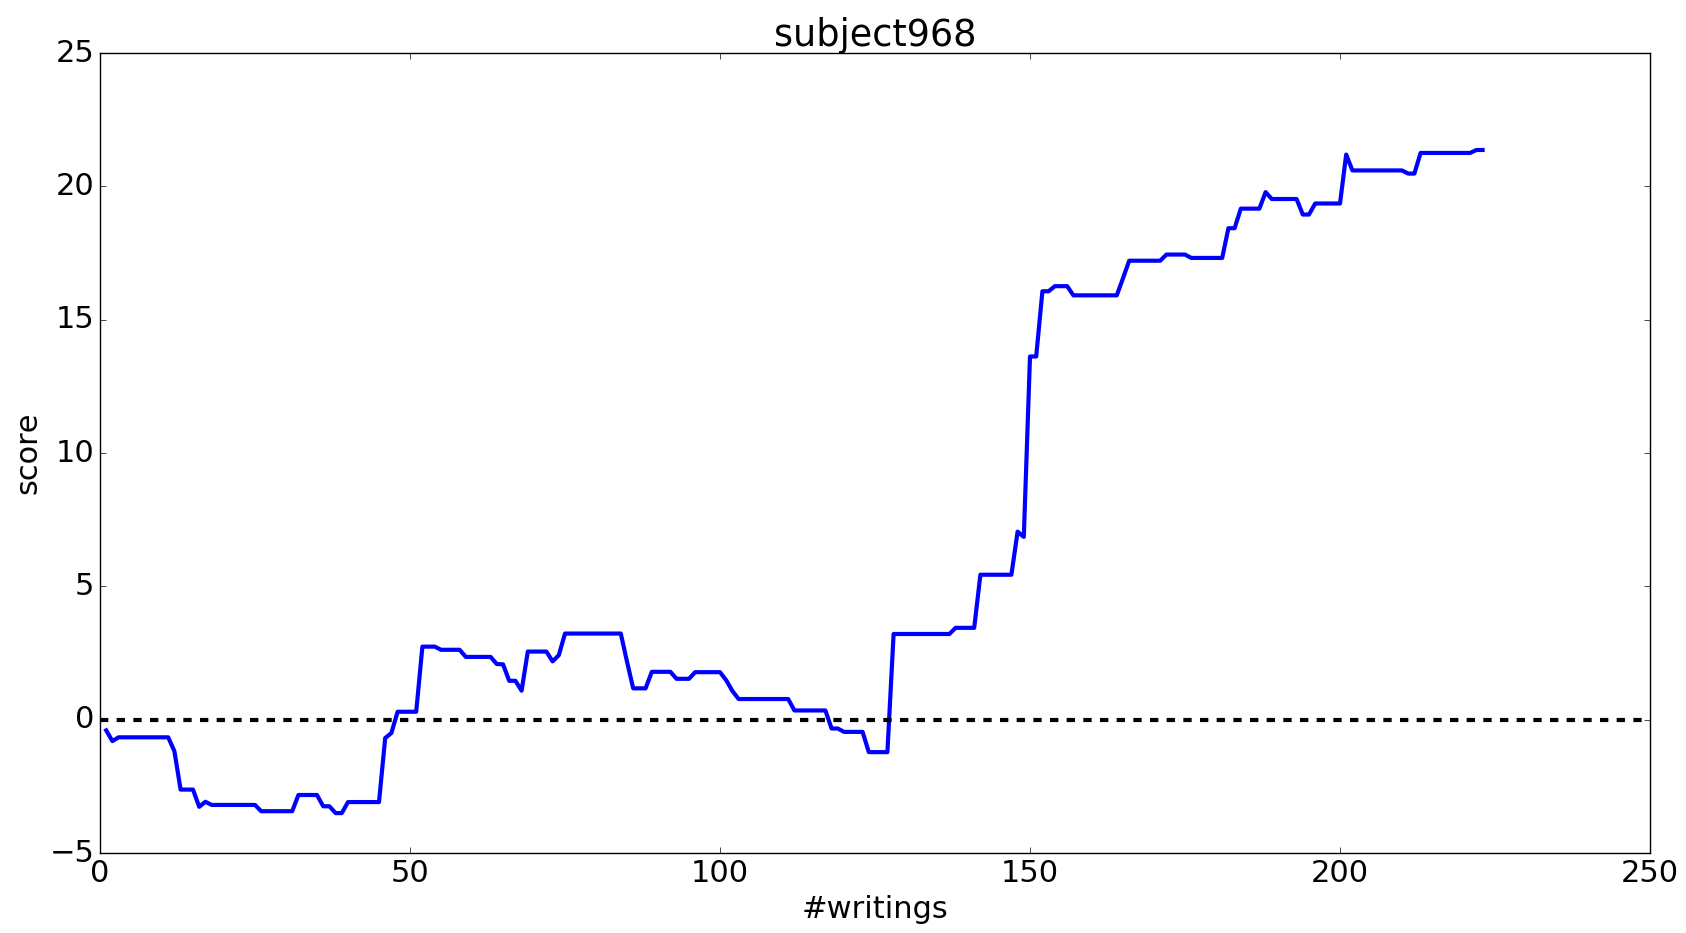
\includegraphics[width=80mm]{images/subject968-score}
        \caption{}
    \end{subfigure}
\caption{
    Sujeto 968 del conjunto de prueba para la tarea de detección anticipada de anorexia.
    (a) Variación del \emph{valor de confianza} positivo y negativo a lo largo del tiempo, publicación a publicación.
    (b) Variación de la \emph{puntuación} estimada ($positivo-negativo$) a lo largo del tiempo, publicación a publicación.
}
\label{fig:subject968}
\end{figure}

% \begin{figure}[t!] % [t]op; [h]ere; [p]age; [b]ottom; [r]ight; [l]eft
%     \centering
%     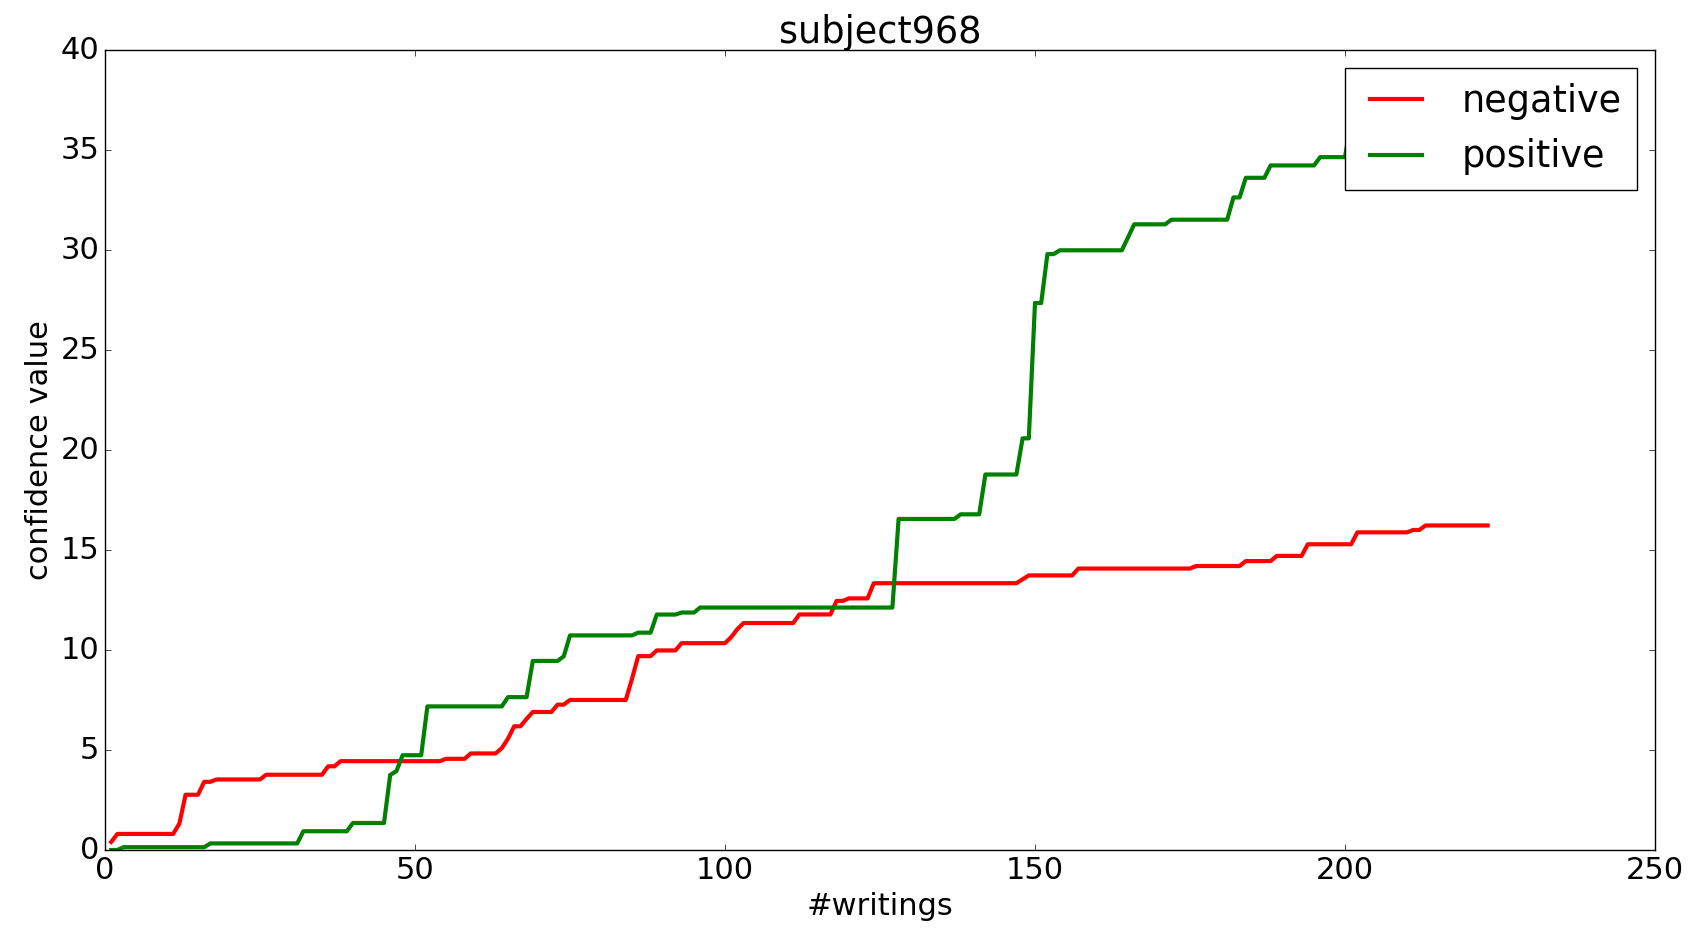
\includegraphics[width=120mm]{images/subject968}
%     \caption{Variación del valor de confianza positivo y negativo del sujeto 968 a lo largo del tiempo (publicaciones).}%Task 3's subject 968's positive and negative confidence value variation over time (writings).
%     \label{fig:subject2341}
% \end{figure}

% \begin{figure}[t!] % [t]op; [h]ere; [p]age; [b]ottom; [r]ight; [l]eft
%     \centering
%     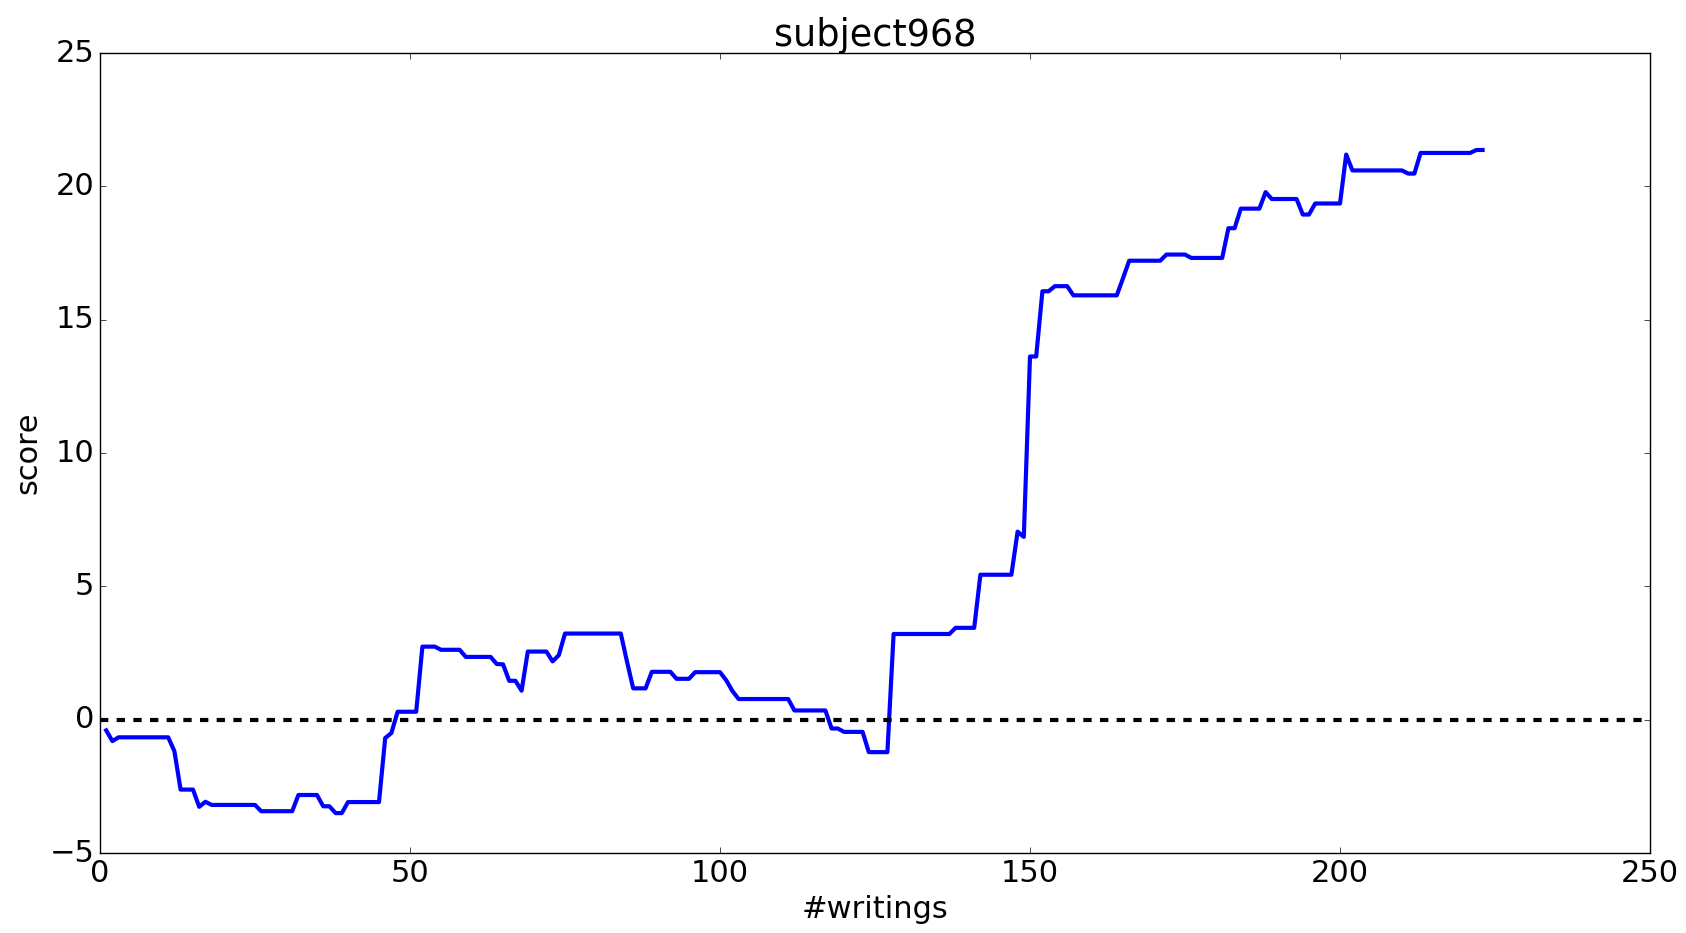
\includegraphics[width=120mm]{images/subject968-score}
%     \caption{Puntuación estimada del nivel de anorexia ($positivo-negativo$) de la tarea 1 del sujeto 968 a lo largo del tiempo (escritos).}%Task 1's subject 968's estimated score of the level of anorexia ($d[positive]-d[negative]$) variation over time (writings).
%     \label{fig:subject2341-cv}
% \end{figure}

% %where $WH_s$ is the subject's writing history. Note that for all the tasks $\overrightarrow{d_s}$ was a vector with two components, one for the positive class and the other for the negative one. The policy to classify a subject as positive was performed analyzing how $\overrightarrow{d_s}$ changed over time, as shown with an example in \autoref{fig:subject2341}. Subjects were classified as positive when the positive value in $\overrightarrow{d_s}$ exceeded the negative one\footnote{Except for task T3 in which we did not perform an "early stop", and therefore every user was classified after processing the entire writing history.}, for instance, the subject in the figure was classified as anorexic after reading the 42nd writing.
% aquí $WH_s$ es la historia de escritura del sujeto. Tenga en cuenta que para todas las tareas $\overrightarrow{d_s}$ era un vector con dos componentes, uno para la clase positiva y el otro para la negativa. La política para clasificar un sujeto como positivo se realizó analizando cómo $\overrightarrow{d_s}$ cambió con el tiempo, como se muestra con un ejemplo en \autoref{fig:subject2341}. Los sujetos fueron clasificados como positivos cuando el valor positivo en $\overrightarrow{d_s}$ excedió al negativo\footnote{Excepto para la tarea T3 en la que no realizamos una "parada temprana", y por lo tanto cada usuario fue clasificado luego de procesar todo el historial de escritura.}, por ejemplo, el sujeto de la figura fue clasificado como anoréxico después de leer el 42º escrito.

%Finally, this year, models performance were also evaluated based on ranking-based measures for tasks T1 and T2. Thus, models were asked to provide an estimated score of the level of anorexia/self-harm along with the binary decision (0/1). To compute this score, SS3 performed the difference between the positive confidence value and the negative one (i.e. $d[positive]-d[negative]$) and returned it along with each decision. For example, in \autoref{fig:subject2341-cv} is shown how this score changed as more writings were read, for the same user shown previously in \autoref{fig:subject2341}.
Como se describió en la sección anterior, en esta edición del eRisk se les pidió a los modelos que, junto con la decisión, proporcionaran una puntuación del nivel de riesgo estimado de cada usuario ---utilizado luego para generar los rankings.
Dicha puntuación fue calculada simplemente considerando la diferencia entre el \emph{valor de confianza} positivo y el negativo, esto es:

\begin{equation}
\text{\emph{puntuación}} = \text{\emph{valor de confianza positivo}} - \text{\emph{valor de confianza negativo}}
\label{eq:puntuacion}
\end{equation}


Como se ilustra con un ejemplo en la \autoref{fig:subject968}, esta simple diferencia permite que, en todo momento, los dos valores de confianza positivo y negativo puedan ser representados por un único valor de confianza unificado, el cual ya no representa el valor de confianza de cada clase, sino más bien un valor de confianza de ``toma de decisión'' que representaría, efectivamente, el nivel de riesgo estimado por el modelo ---ya que es el valor utilizado por el modelo para, efectivamente, clasificar y detectar a los usuarios en riesgo.


\section{Tareas y Resultados Obtenidos}

Esta sección describe la participación en el eRisk 2019 con los modelos propuestos en los capítulos anteriores. En las siguientes secciones se describe cada tarea  y se examinan los resultados obtenidos en cada una de las mismas.


\subsection{Tarea 1: Detección Anticipada de Anorexia}%Task 1: Early Detection of Signs of Anorexia

\begin{table*}[t]
\centering
\caption{Estadísticas principales del conjunto de datos de la tarea 1.}
\label{tab:dataset-t1}
\begin{tabular}{l c c|c c}
\hline
& \multicolumn{2}{c}{Entrenamiento} & \multicolumn{2}{c}{Prueba}\\
& Anorexia & Control & Anorexia & Control \\ \hline
No. de sujetos & 61 & 411 & 73 & 742 \\
No. de publicaciones & 24874 & 228878 & 17619 & 552890 \\
Prom. de publicaciones por sujeto & 407.8 & 556.9 & 241.4 & 745.1 \\
Prom. de días (primera a última publ.) & 800 & 650 & 510 & 930 \\
Prom. de palabras por publicación & 37.3 & 20.9 & 37.2 & 21.7 \\ \hline

\hline
\end{tabular}
\end{table*}


En esta tarea participaron un total de 13 equipos de investigación distintos y se enviaron un total de 50 modelos distintos.
Como se describe más detalladamente en la descripción general del eRisk~\cite{losadaetal2019}, esta tarea se planteó como una continuación de la tarea de detección anticipada de anorexia del eRisk 2018, por lo que, en esta nueva edición, el conjunto de entrenamiento se conformó uniendo el conjunto de entrenamiento y el de prueba de esa edición.
La evaluación de los modelos se llevó a cabo utilizando un nuevo conjunto de prueba construido con la misma metodología que en las ediciones anteriores, es decir, recolectando las publicaciones de un conjunto de usuarios de Reddit divididos en dos grupos, aquellos diagnosticados con anorexia y aquellos que no.
En la \autoref{tab:dataset-t1} se brindan las principales estadísticas del conjunto de datos completo, en donde se puede observar que, nuevamente, las clases están altamente desbalanceadas ---por ejemplo, sólo $73$ de los $815$ usuarios del conjunto de prueba están etiquetados como en riesgo.


\

La participación en esta tarea se llevó a cabo utilizando $5$ modelos distintos, los cuales fueron nombrados dentro del eRisk respectivamente como \emph{UNSL\#0, UNSL\#1, UNSL\#2, UNSL\#3, UNSL\#4}.\footnote{Los nombres de los modelos participantes fueron conformados por el nombre registrado para su equipo, en nuestro caso ``UNSL'', seguido de un \# y su respectivo número.} 
Como se detalló en la \autoref{sec:erisk2019implementacion}, se utilizaron los mismos valores de hiperparámetros para los $5$ modelos. Por lo tanto, la principal diferencia entre cada uno de estos modelos estuvo dada por la manera en la que fueron entrenados y el tipo específico de modelo SS3 utilizado, como se detalla a continuación:

\begin{itemize}
\item \emph{UNSL\#0}: modelo SS3 original entrenado con el conjunto de entrenamiento del eRisk 2018, excluyéndose así del entrenamiento a los usuarios correspondientes al conjunto de prueba de esa misma edición.
De esta manera, el modelo obtenido se correspondió al utilizado en el capítulo anterior, permitiendo evaluar la consistencia y robustez de los resultados en relación a los obtenidos previamente en la experimentación controlada.
\item \emph{UNSL\#1}: análogo al modelo anterior pero utilizando $\tau$-SS3 en lugar de SS3.
% este modelo es el mismo que el anterior pero permitiendo que SS3 reconozca bigramas de palabras.
\item \emph{UNSL\#2}: modelo SS3 entrenado utilizando el conjunto de entrenamiento completo disponible para esta edición. Esto es, el modelo se entrenó utilizando tanto los usuarios del conjunto del entrenamiento como los de prueba del eRisk 2018.
\item \emph{UNSL\#3}: análogo al modelo anterior pero utilizando $\tau$-SS3 en lugar de SS3.
\item \emph{UNSL\#4}: modelo UNSL\#2 modificado para que, durante el proceso de clasificación, sólo se tengan en cuenta las palabras con un \emph{valor global} mayor a $0.3$ ---\emph{i.e.} SS3 asignó $gv(w, c_i) = 0$ a todo $w$ y $c_i$ tal que $gv(w, c_i)\leq0.3$.\footnote{Utilizando los datos del conjunto de entrenamiento se probaron, comenzando en $0$, incrementalmente distintos valores, eligiéndose así $0.3$ por haber obtenido el mejor valor $ERDE_{50}$.}
Con esta variante se intentó medir qué impacto tienen las palabras con bajo \emph{valor global} en el desempeño de clasificación, es decir, con este modelo se buscó abordar preguntas tales como: ``¿qué tan sensible es el modelo al ruido que podrían introducir la gran cantidad de palabras con un \emph{valor global} bajo?'' o ``¿podría ser el caso de que a causa de estas palabras la condición de clasificación anticipada se dispare incorrectamente producto del ruido acumulado al procesarlas?''.
% Este modelo obtuvo el mejor valor $ERDE_{50}$.
% con esta variante se buscó evitar que el modelo sea demasiado sensible al ruido que podrían introducir palabras con un \emph{valor global} bajo.
% La hipótesis fue que estas palabras con bajo \emph{valor global} podrían causar que la condición de clasificación anticipada se dispare incorrectamente producto del ruido acumulado al procesarlas.
\end{itemize}


\vspace{5mm}

A continuación se presentarán los resultados obtenidos para esta tarea,
sin embargo, es adecuado mencionar previamente que a ninguno de los participantes se le permitió optimizar sus modelos en relación a las nuevas medidas, ya que las mismas sólo se dieron a conocer junto con la publicación de los resultados finales.
Así, los principales resultados obtenidos con los 5 modelos descritos anteriormente, agrupados según las medidas utilizadas para medir el desempeño de los mismos, son los siguientes:
% Estos resultados son presentados en tres grupos distintos dependiendo del desempeño medido, uno para las medidas centradas en la decisión,  como las basadas en ranking, se podrían resumir de la siguiente manera:

% Los principales resultados globales obtenidos en esta tarea, tanto para las medidas centradas en la decisión como las basadas en ranking, se podrían resumir de la siguiente manera:

\begin{table*}[t!]
\centering
\caption{Resultados obtenidos en la tarea 1 para las medidas centradas en la decisión. A modo de comparación, del total de 50 modelos participantes, aquí se muestran, ordenados por $ERDE_{50}$, sólo los modelos que obtuvieron los mejores valores de cada uno de los otros 12 equipos de investigación.}
\label{tab:t1-result}
\begin{tabular}{l c c c c c c c c c c}
\hline
% Team\#run & P & R & $F1$ & $F2$ & $ERDE_5$ & $ERDE_{50}$ & $F_{latency}$ & $F2_{latency}$ \\
Equipo\#modelo & $ERDE_5$ & $ERDE_{50}$ & $F_{latency}$\\ \hline

UNSL\#0 & \textbf{5.53\%} & 3.92\% & .55 \\
UNSL\#1 & 5.68\% & 4.10\% & .55 \\
UNSL\#2 & 5.56\% & 3.34\% & .50 \\
UNSL\#3 & 5.59\% & 3.48\% & .49 \\
UNSL\#4 & 6.14\% & \textbf{2.96\%} & .46 \\
\hline
\hline
CLaC\#1 & 5.73\% & 3.13\% & \textbf{.69} \\
BiTeM\#1 & 5.89\% & 3.40\% & .54 \\
CLaC\#4 & 6.25\% & 3.42\% & \textbf{.69} \\
UDE\#0 & 8.48\% & 3.87\% & .58 \\
UDE\#1 & 7.48\% & 3.94\% & .53 \\
INAOE-CIMAT\#0 & 9.29\% & 3.98\% & .62 \\
LTL-INAOE\#1 & 7.74\% & 4.20\% & .55 \\
INAOE-CIMAT\#3 & 9.17\% & 4.75\% & .63 \\
SINAI\#2 & 9.04\% & 4.89\% & .30 \\
INAOE-CIMAT\#4 & 9.12\% & 5.07\% & .61 \\
lirmm\#0 & 9.13\% & 5.14\% & .63 \\
UppsalaNLP\#4 & 5.73\% & 5.66\% & .41 \\
BioInfo@UAVR\#0 & 5.84\% & 5.77\% & .37 \\
lirmm\#3 & 9.08\% & 6.62\% & .48 \\
SSN-NLP\#3 & 7.61\% & 6.86\% & .33 \\
HULAT\#0 & 10.84\% & 8.14\% & .16 \\
UDE\#2 & 12.52\% & 8.21\% & .53 \\
Fazl\#2 & 17.11\% & 11.22\% & .14 \\
Fazl\#1 & 17.11\% & 13.91\% & .11 \\

\hline
\end{tabular}
\end{table*}

% \begin{table*}[t!]
% \centering
% \caption{Resultados de la Tarea 1, evaluación basada en decisiones. Los mejores resultados de cada uno de los 13 equipos también se muestran para comparar.}%Results for Task 1, decision-based evaluation. Best results are also shown for comparison.
% \label{tab:t1-result}
% \begin{tabular}{l c c c c c c c c c c}
% \hline
% % Team\#run & P & R & $F1$ & $F2$ & $ERDE_5$ & $ERDE_{50}$ & $F_{latency}$ & $F2_{latency}$ \\
% Team\#run & P & R & $F1$ & $ERDE_5$ & $ERDE_{50}$ & $F_{latency}$ & $F2_{latency}$ \\ \hline

% % BiTeM\#1 & .44 & .70 & .54 &  & .06 & .03 & .54 \\
% UDE\#0 & .51 & .74 & .61 & 8.48\% & 3.87\% & .58 & .64 \\
% lirmm\#1 & \textbf{.77} & .60 & .68 & 9.09\% & 5.50\% & .62 & .57 \\
% lirmm\#2 & .66 & .70 & .68 & 9.24\% & 5.80\% & .60 & .60 \\
% Fazl\#2 & .09 & \textbf{1} & .16 & 17.11\% & 11.22\% & .14 & .28 \\
% CLaC\#0 & .45 & .74 & .56 & 6.72\% & 3.93\% & .54 & .63 \\
% CLaC\#1 & .61 & .82 & .70 & 5.73\% & 3.12\% & .69 & \textbf{.75} \\
% CLaC\#2 & .60 & .81 & .69 & 6.01\% & 3.13\% & .68 & .73 \\
% CLaC\#3 & .63 & .81 & .69 & 6.27\% & 3.54\% & .68 & .74 \\
% CLaC\#4 & .64 & .79 & \textbf{.71} & 6.25\% & 3.42\% & \textbf{.69} & .73 \\
% LTL-INAOE\#1 & .47 & .75 & .58 & 7.74\% & 4.19\% & .55 & .64 \\
% INAOE-CIMAT\#0 & .56 & .78 & .66 & 9.29\% & 3.98\% & .62 & .68 \\
% INAOE-CIMAT\#3 & .67 & .68 & .68 & 9.17\% & 4.75\% & .63 & .69 \\
% INAOE-CIMAT\#4 & .69 & .63 & .66 & 9.12\% & 5.07\% & .61 & .59 \\
% UNSL\#0 & .42 & .78 & .55 & \textbf{5.53\%} & 3.92\% & .55 & .66 \\
% UNSL\#1 & .43 & .75 & .55 & 5.68\% & 4.10\% & .55 & .65 \\
% UNSL\#2 & .36 & .86 & .51 & 5.56\% & 3.34\% & .50 & .67 \\
% UNSL\#3 & .35 & .85 & .50 & 5.59\% & 3.48\% & .49 & .66 \\
% UNSL\#4 & .31 & .92 & .47 & 6.14\% & \textbf{2.96\%} & .46 & .65 \\

% % UDE\#0 & .51 & .74 & .61 & .67 & .08 & .04 & .58 & .64 \\
% % lirmm\#1 & \textbf{.77} & .60 & .68 & .62 & 9.xx\% & 6.xx\% & .62 & .57 \\
% % lirmm\#2 & .66 & .70 & .68 & 69 & .09 & .06 & .60 & .60 \\
% % Fazl\#2 & .09 & \textbf{1} & .16 & .33 & 17.xx\% & 11.xx\% & .14 & .28 \\
% % CLaC\#0 & .45 & .74 & .56 & .65 & .07 & .04 & .54 & .63 \\
% % CLaC\#1 & .61 & .82 & .70 & .76 & .06 & .03 & .69 & .75 \\
% % CLaC\#2 & .60 & .81 & .69 & .75 & .06 & .03 & .68 & .73 \\
% % CLaC\#3 & .63 & .81 & .69 & .76 & .06 & .03 & .68 & .74 \\
% % CLaC\#4 & .64 & .79 & \textbf{.71} & .75 & 6.xx\% & 3.xx\% & \textbf{.69} & .73 \\
% % LTL-INAOE\#1 & .47 & .75 & .58 & .67 & .08 & .04 & .55 & .64 \\
% % INAOE-CIMAT\#0 & .56 & .78 & .66 & .72 & .09 & .04 & .62 & .68 \\
% % INAOE-CIMAT\#3 & .67 & .68 & .68 & .75 & .09 & .05 & .63 & .69 \\
% % INAOE-CIMAT\#4 & .69 & .63 & .66 & .64 & .09 & .05 & .61 & .59 \\
% % UNSL\#0 & .42 & .78 & .55 & .66 & \textbf{6.xx\%} & 4.xx\% & .55 & .66 \\
% % UNSL\#1 & .43 & .75 & .55 & .65 & 6.xx\% & 4.xx\% & .55 & .65 \\
% % UNSL\#2 & .36 & .86 & .51 & .67 & 6.xx\% & 3.xx\% & .50 & .67 \\
% % UNSL\#3 & .35 & .85 & .50 & .66 & 6.xx\% & 3.xx\% & .49 & .66 \\
% % UNSL\#4 & .31 & .92 & .47 & .66 & 6.xx\% & \textbf{3.xx\%} & .46 & .65 \\

% \hline
% \end{tabular}
% \end{table*}

\begin{itemize}
% UNSL0  ---en relación a los siguientes modelos, éste obtuvo los mejores valores $ERDE_5$ y $F_{latency}$
    \item \textbf{Desempeño centrado en la decisión:} en la \autoref{tab:t1-result} se muestran los resultados obtenidos para las medidas centradas en la decisión.
    En relación a las medidas $ERDE$, se puede observar que el modelo \emph{UNSL\#0} obtuvo el mejor $ERDE_5$ y el \emph{UNSL\#4} el mejor $ERDE_{50}$, no obstante, este último fue el que obtuvo el peor valor $F_{latency}$ de entre los 5 modelos.
    Esto último sugiere que ignorar las palabras con bajo \emph{valor global} puede, de hecho, contribuir a mejorar el desempeño en términos de la medida $ERDE$ pero a costa de un peor desempeño en términos de la medida $F_{latency}$ ya que, en relación al original, el modelo resultante prioriza aún más $recall$ por sobre $precision$,\footnote{\emph{UNSL}\#4 obtuvo el mejor $recall$ ($0.92$) pero el valor $precision$ más bajo ($0.31$).} lo que finalmente afecta la media armónica de estas últimas.
    Los modelos \emph{UNSL\#2} y \emph{\#3} entrenados con el conjunto de entrenamiento completo obtuvieron un mejor desempeño en términos de la medida $ERDE_{50}$ en relación a sus dos contrapartes, \emph{UNSL\#0} y \emph{\#1}, entrenadas sólo con el conjunto de entrenamiento correspondiente a la edición anterior del eRisk ---e.d. los mismos modelos utilizados en el capítulo anterior.
    Sin embargo, el desempeño de estos modelos en términos de la nueva medida $F_{latency}$ fue menor en relación al de estos últimos, esto probablemente se deba a que los hiperparámetros utilizados ajustan el modelo al conjunto de datos en relación a la medida $ERDE_{50}$ ---nuevamente priorizando el $recall$ por sobre su media armónica con la medida $precision$.
    A diferencia de los resultados obtenidos en el capítulo anterior, ambos modelos $\tau$-SS3 (\emph{UNSL\#1 y \#3}) obtuvieron un desempeño ligeramente menor a sus contrapartes utilizando SS3 (respectivamente, \emph{UNSL\#0 y \#2}) con este conjunto de datos.
    Esto tal vez se deba a que el uso de \emph{n-gramas} si bien puede tener cualidades semánticas superiores con respecto a la bolsa de palabras, también sufre de cualidades estadísticas inferiores\footnote{La probabilidad con la que aparece una secuencia de palabras nunca será mayor que la probabilidad individual de cada palabra.} lo que, dependiendo del conjunto de datos utilizado, puede afectar negativamente al desempeño.
    Además, a diferencia del capítulo anterior, aquí los usuarios fueron procesados publicación a publicación y no utilizando los \emph{bloques} de publicaciones ---en donde hasta incluso el modelo más apresurado debió procesar al menos un bloque completo antes de poder tomar una decisión.
    En relación a la nueva medida $F_{latency}$, ninguno de los 5 modelos obtuvo un resultado destacable ya que el mejor valor obtenido ($0.55$), correspondiente a \emph{UNSL\#0} y \emph{\#1}, estuvo $0.13$ puntos por debajo del mejor valor, obtenido por \emph{CLaC\#4} ---del cual se hablará en el siguiente apartado.
    Este resultado se debe principalmente a que, como se mencionó, los 5 modelos utilizaron los mismos valores de hiperparámetros utilizados en los capítulos anteriores, los cuales fueron seleccionados optimizando la medida $ERDE$.
    Por lo tanto, como se explicó al final de la \autoref{sec:medidas_decision}, los modelos resultantes priorizaron tanto el $recall$ como la velocidad.\footnote{En promedio, los 5 modelos SS3 clasificaron a los usuarios en riesgo luego de procesar solamente la segunda o tercera publicación de cada uno de ellos.}
    No obstante, el mejor valor $F_{latency}$ obtenido ($0.55$) se encuentra considerablemente por encima del promedio ($0.38$), ubicándose en el puesto 11 de entre los 50 modelos participantes.
\begin{table*}[t!]
\centering
%\caption{Participating teams for Task 1: number of runs, number of user writings processed by the team, and the time taken for the whole process and for processing each writing (i.e $\frac{TotalTime}{\#writings\times\#runs}$). (*) This value was originally 5, but we replaced it by the actual number of models used.}
\caption{Detalle de los equipos participantes en la tarea 1: nombre del equipo, cantidad de modelos empleados ($\#modelos$), número de publicaciones procesadas de los usuarios ($\#publicaciones$), tiempo total empleado para completar la tarea y tiempo empleado para procesar cada publicación (\emph{i.e.} $\frac{tiempo\ total}{\#publicaciones\times\#modelos}$).}
\label{tab:t1-time}
\begin{tabular}{l c c|c | c}
\hline
& & & \multicolumn{2}{c}{Tiempo} \\
Equipo & \#modelos & \#publicaciones & total & por publicación  \\ \hline

\textbf{UNSL}$\star$ & 5 & 2000 & 23h & \textbf{8s} \\
UppsalaNLP & 5 & 2000 & 2 días + 7h & 20s \\
BioInfo@UAVR & 1 & 2000 & 14h & 25s \\
UDE & 3 & 2000 & 5 días + 3h & 1m + 12s \\
lirmm & 5 & 2024 & 8 días + 15h & 1m + 12s \\
INAOE-CIMAT & 4 & 2000 & 8 días + 2h & 1m + 30s \\
HULAT & 5 & 83 & 18h & 2m + 36s \\
Fazl & 3 & 2001 & 21 días + 15h & 5m + 12s \\
BiTeM & 4 & 11 & 4h & 5m + 30s \\
LTL-INAOE & 2 & 2001 & 17 días + 23h & 6m + 30s \\
SINAI & 3 & 317 & 10 días + 7h & 15m + 36s \\
CLaC & 5 & 109 & 11 días + 16h & 31m \\
SSN-NLP & 5 & 9 & 6 días + 22h & 3h + 42m \\

\hline
\end{tabular}
\end{table*}

    \item \textbf{Desempeño en relación al tiempo de ejecución:} en la \autoref{tab:t1-time} se muestran, por cada equipo, detalles sobre el tiempo total empleado para completar la tarea.
    Como se puede observar, el tiempo tomado para completar la tarea difiere ampliamente de equipo en equipo, variando desde unas pocas hasta una gran cantidad de horas ---en un caso incluso llegando hasta cerca de un mes.
    Sin embargo, para tener una visión más precisa de qué tan eficientes fueron los modelos de cada equipo, no sólo se debe tener en cuenta el tiempo total empleado para completar la tarea sino también la cantidad de publicaciones procesadas en ese tiempo, y el número de modelos utilizados para llevarlo a cabo.
    Por ejemplo, en términos de velocidad de procesamiento, no sería igual de eficiente BiTeM que UNSL, ya que si bien el primero completó la tarea en 4 horas, sólo procesó las primeras 11 publicaciones de cada usuario, mientras que el segundo, si bien demoró 23 horas, procesó la totalidad de las 2000 publicaciones disponibles para cada uno de ellos.
    De la misma manera, no sería igual de eficiente BioInfo@UAVR que UNSL, ya que si bien el primero demoró 14 horas en clasificar a todos los usuarios con un único modelo, el segundo lo tuvo que realizar con 5 de ellos, lo que implicó no sólo un procesamiento 5 veces mayor sino también el envío de 5 veces más peticiones hacia el servidor.\footnote{Por cada una de las 2000 publicaciones no sólo se necesitó una petición para obtener la publicación, sino también se necesitaron 5 peticiones para enviar la respuesta de cada uno de los 5 modelo. Por lo tanto, para grupos como UNSL, completar la tarea requirió de un total de $2000 + 2000*5 = 12000$ peticiones al servidor. Por lo tanto, si la latencia de conexión fue de, por ejemplo, 3 segundos, se tiene que aproximadamente 10 horas del total fueron consumidos sólo en la comunicación.}
    Por este motivo, en la \autoref{tab:t1-time} también se incluye una estimación del tiempo que le tomó a los modelos procesar cada publicación, el cual se obtuvo normalizando el tiempo total en relación a la cantidad de modelos utilizados y el número de publicaciones procesadas por cada uno de ellos.
    Así, se puede observar que UNSL fue el equipo más eficiente en términos de tiempos de ejecución, habiendo procesado cada publicación en aproximadamente 8 segundos\footnote{Ya que este tiempo incluye la latencia de recibir la publicación, el tiempo utilizado efectivamente para procesarla, y luego la latencia del envío de la respuesta, gran parte de estos 8 segundos se corresponden a dichas latencias.} ---\emph{i.e.} 2000 publicaciones de cada usuario procesadas con 5 modelos en 23 horas.
    Vale la pena mencionar que el hecho de que UNSL haya sido el más rápido en procesar cada publicación no se debió a la utilización de un poder de cómputo superior al del resto de los participantes para ejecutar sus modelos,\footnote{Para ejecutar el script Python con los modelos se utilizó la computadora portátil personal del autor del presente documento, la cual tiene especificaciones técnicas ordinarias, por ejemplo, un procesador Intel Core i5 y 8GB de RAM.} sino a la utilización del modelo SS3 que, como vimos en el \autoref{cap:ss3}, fue diseñado para poder trabajar incrementalmente, permitiéndole procesar la secuencia (de publicaciones) de entrada en tiempo de orden $O(n)$, con respecto al largo de la misma.
    Esto contrasta con otros equipos, tales como CLaC~\cite{mohammadi2019quick}, INAOE-CIMAT~\cite{aragon2019inaoe} o lirmm~\cite{ragheb2019attentive}, que si bien obtuvieron un mejor desempeño en relación a, por ejemplo, la medida $F_{latency}$, fueron considerablemente más lentos, tomándole días completar la misma tarea.
    Por ejemplo, los 5 modelos de CLaC~\cite{mohammadi2019quick} emplearon un clasificador \ac{SVM} que tomaba como entrada una representación vectorial obtenida ensamblando varios modelos neuronales basados en mecanismos de atención, uno de los cuales (\emph{CLaC\#1}) obtuvo el mejor valor $F_{latency}$.
    Sin embargo, estos modelos fueron 232 veces más lentos que los modelos SS3 de UNSL, ya que a CLaC le tomó 11 días y 16 horas procesar sólo 109 publicaciones ---lo que podría indicar que los modelos utilizados fueron sustancialmente ineficientes, en términos computacionales. %, o incluso podría sugerir que algunos grupos de investigación incorporaron algún tipo de intervención manual en sus modelos.


\begin{table*}[t!]
\caption{Resultados obtenidos en la tarea 1 para las medidas basadas en ranking para 4 rankings distintos, respectivamente, el ranking obtenido luego de leer 1, 100, 500 y 1000 publicaciones. Aquí también se incluyen, a modo de comparación, los mejores resultados obtenidos por los otros 12 equipos.}
\label{tab:t1-result-ranking}
\centering{
\begin{tabular}{l c c c|c c c}
\hline
& \multicolumn{3}{c}{1 publicación leída} & \multicolumn{3}{c}{100 publicaciones leídas} \\
Equipo\#modelo & P@10 & NDCG@10 & NDCG@100 &  P@10 & NDCG@10 & NDCG@100 \\ \hline
UNSL\#0 & \textbf{.8} & \emph{\textbf{.82}} & .54 & \textbf{1} & \textbf{1} & .77 \\
UNSL\#1 & \textbf{.8} & \emph{\textbf{.82}} & .54 & \textbf{1} & \textbf{1} & .77 \\
UNSL\#2 & \textbf{.8} & \emph{\textbf{.82}} & \emph{\textbf{.55}} & \textbf{1} & \textbf{1} & .83 \\
UNSL\#3 & \textbf{.8} & \emph{\textbf{.82}} & .53 & \textbf{1} & \textbf{1} & .83  \\
UNSL\#4 & \textbf{.8} & \emph{\textbf{.82}} & .52 & .9 & .94 & \emph{\textbf{.85}} \\
\hline\hline
LTL-INAOE\#0 & \textbf{.8} & .75 & .34 & \textbf{1} & \textbf{1} & .76 \\
UDE\#1 &  .6 & .75 & .54 & .9 & .94 & .81 \\
UppsalaNLP\#4 &  .8 & .75 & .52 & .8 & .75 & .52 \\
BiTeM\#1 &  .8 & .75 & .47 & - & - & - \\
SSN-NLP\#3 &  .6 & .64 & .3 & - & - & - \\
BioInfo@UAVR\#0 &  .6 & .59 & .47 & .6 & .59 & .47 \\
BiTeM\#0 &  .6 & .44 & .52 & - & - & - \\
HULAT\#0 &  .3 & .33 & .18 & - & - & - \\
Fazl\#1 &  .3 & .29 & .26 & .6 & .6 & .59 \\
UDE\#0 &  .2 & .12 & .11 & .9 & .92 & .81 \\
SINAI\#0 &  .2 & .12 & .11 & - & - & - \\
CLaC\#0 &  .1 & .1 & .05 & .8 & .86 & .28 \\
CLaC\#1 &  .1 & .1 & .04 & .3 & .45 & .16 \\
\hline
\hline
\end{tabular}


\

\


\begin{tabular}{l c c c|c c c}
\hline
& \multicolumn{3}{c}{500 publicaciones leídas} & \multicolumn{3}{c}{1000 publicaciones leídas} \\
Equipo\#modelo & P@10 & NDCG@10 & NDCG@100 &  P@10 & NDCG@10 & NDCG@100 \\ \hline
UNSL\#0 & \textbf{1} & \textbf{1} & .79 & \textbf{1} & \textbf{1} & .79 \\
UNSL\#1 & \textbf{1} & \textbf{1} & .79 & \textbf{1} & \textbf{1} & .79 \\
UNSL\#2 & \textbf{1} & \textbf{1} & .83 & \textbf{1} & \textbf{1} & \emph{.84} \\
UNSL\#3 & \textbf{1} & \textbf{1} & .84 & \textbf{1} & \textbf{1} & \emph{.84}  \\
UNSL\#4 & \textbf{1} & \textbf{1} & \emph{.85} & .9 & .94 & \emph{.84} \\
\hline\hline
UDE\#1 &  \textbf{1} & \textbf{1} & \textbf{.87} & \textbf{1} & \textbf{1} & \textbf{.88} \\
UDE\#0 &  .9 & .93 & \emph{.85} & .9 & .94 & .86 \\
LTL-INAOE\#0 & .9 & .92 & .73 & .7 & .78 & .65 \\
Fazl\#1 &  .7 & .78 & .67 & .7 & .78 & .68 \\
UppsalaNLP\#4 &  .8 & .75 & .52 & .8 & .75 & .52 \\
BioInfo@UAVR\#0 &  .6 & .59 & .47 & .6 & .59 & .47 \\

\hline
\hline
\end{tabular}}

\end{table*}

    \item \textbf{Desempeño basado en ranking:} en la \autoref{tab:t1-result-ranking} se muestran los resultados obtenidos para las medidas basadas en ranking.\footnote{La ausencia de algunos modelos simplemente se debe a que no enviaron la \emph{puntuación} solicitada o bien no procesaron la mínima cantidad de publicaciones necesaria para el respectivo ranking.}
    Se puede observar que los 5 modelos SS3 obtuvieron, en los 4 rankings, los mejores valores para las medidas $P@10$ y $NDCG@10$.
    Además, en relación a la medida $NDCG@100$, se obtuvieron los mejores valores para los rankings obtenidos luego de procesar $1$ y $100$ publicaciones, y el segundo y tercer mejor valor para los rankings obtenidos, respectivamente, luego de procesar $500$ y $1000$ publicaciones.
    % Además, para el ranking obtenido luego de procesar $500$ publicaciones, \emph{UNSL\#4} obtuvo el segundo mejor $NDCG@100$ con $.85$ (siendo $.87$ el mejor valor) y el tercer mejor $NDCG@100$ con $.84$ (siendo $.88$ el mejor) para el ranking luego de $1000$ publicaciones. \footnote{Estos mejores valores de $NDCG@100$ fueron obtenidos por UDE\#1~\cite{masood2019ude}. Vale la pena mencionar que a UDE le tomó 1 día y 6 horas procesar esas 500 publicaciones (y 2 días y 12 horas para las 1000) mientras que SS3 tardó sólo 5 horas en procesarlas, siendo por lo tanto 9 veces más rápido pero sólo teniendo un desempeño ligeramente menor en términos de $NDCG@100$ (una diferencia de apenas $0.02$ y $0.04$, respectivamente).}
    % Diferencia entre los distintos modelos UNSL:
    En relación al desempeño de las distintas variantes utilizadas, no hubo una diferencia perceptible entre los modelos SS3 (UNSL\#0 y \#2) y sus contrapartes $\tau$-SS3 (UNSL\#1 y \#3).
    Entre los modelos entrenados sólo con el conjunto de entrenamiento del eRisk 2018 (UNSL\#0 y \#1) y los entrenados con todo el conjunto de entrenamiento (UNSL\#2, \#3 y \#4) tampoco hubo una diferencia en términos de las medidas $P@10$ y $NDCG@10$, sin embargo, en términos de la medida $NDCG@100$, los modelos entrenados con todo el conjunto de datos fueron considerablemente mejores.
    Esto es, el haber usado todas las instancias de entrenamiento mejoró la capacidad de los modelos de estimar el nivel de riesgo de los usuarios ---por ejemplo, el ranking de 100 usuarios generado con las estimaciones dadas por UNSL\#0, con 100 publicaciones leídas, fue un 77\% ideal\footnote{En esta tarea, el ranking ideal es el ranking en donde todos los 73 usuarios en riesgo están ubicados en las primeras 73 posiciones.} (i.e. su $NDCG@100$ fue de $0.77$), mientras que el obtenido con UNSL\#2 fue un 83\% ideal.
    % En relación al ignorar las palabras con valores globales bajos, los resultados obtenidos con UNSL\#4 sugieren que podrían tener una leve mejora en relación en NDCG@100, pero tuvo un impacto ligeramente negativo en las medidas P@10 y NDCG@10
    En líneas generales se puede observar que, de entre todos los modelos participantes, las estimaciones de riesgo de los 5 modelos SS3, y sus variantes, fueron las más consistentes a lo largo de todos los rankings, en donde se obtuvieron los mejores valores incluso cuando el ranking fue generado luego de leer sólo la primer publicación de cada usuario.
    Por ejemplo, en relación a este último punto, es interesante notar que, independientemente de si fueron entrenados con el conjunto de entrenamiento completo o si se tuvieron en cuenta transiciones de palabras o no, todos los modelos SS3 fueron capaces de construir un ranking de 10 usuarios en riesgo que fue 82\% ideal (i.e. $NDCG@10 = 0.82$) con sólo 1 publicación leída de cada usuario.
    Esto nos indica que los modelos, a pesar de su relativa simpleza, son capaces de estimar el nivel de riesgo de los usuarios con una eficiencia considerable, aún cuando se han leído unas pocas publicaciones ---lo que explicaría por qué, a pesar de haber clasificado a los usuarios en riesgo luego de haber procesado, en promedio, tan solo 3 de sus publicaciones, no se obtuvo un mal desempeño de clasificación anticipada.
    Esto contrasta con otros modelos más complejos que, si bien obtuvieron un mejor desempeño en la medida $F_{latency}$, no fueron tan eficientes en estimar el nivel de riesgo de los usuarios a pesar de haber demorado días en completar la tarea ---por ejemplo, si bien el modelo CLaC\#1 obtuvo el mejor valor $F_{latency}$, su capacidad de estimar el nivel de riesgo de los usuarios fue la más baja de entre todos los modelos participantes, a pesar de haber demorado más de 11 días en completar la tarea.
    \begin{figure}[t!]
    \centering
    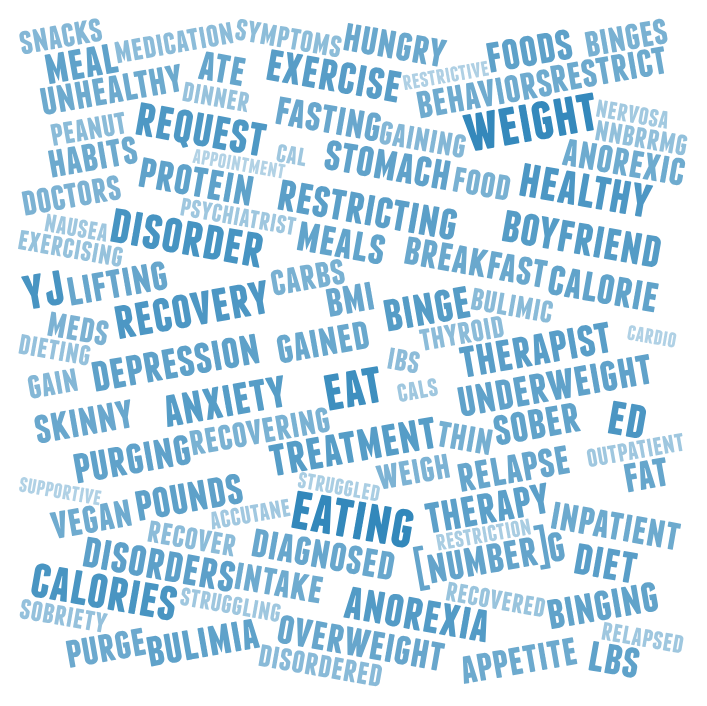
\includegraphics[width=.7\textwidth]{images/anorexia(gv)}
    \caption{Top 100 palabras seleccionadas por el \emph{valor global} aprendido para la clase positiva (anorexia) de la tarea 1.
    El tamaño de cada palabra se corresponde con su respectivo valor.}
    \label{fig:word-cloud-t1}
    \end{figure}
    Finalmente, es importante mencionar que estos resultados implican dos puntos relevantes: (a) la \emph{puntuación}\footnote{Véase \autoref{eq:puntuacion}.} generada por SS3 está estimando el nivel de riesgo de los sujetos correctamente, en otras palabras, efectivamente el \emph{valor global}, dado por $gv(w, c)$, está capturando correctamente el grado de importancia de las palabras ---lo que también se puede comprobar desde un punto de vista más cualitativo, como en los capítulos anteriores, por medio de una nube de palabras como la mostrada en la \autoref{fig:word-cloud-t1}; y más importante aún, (b) el hecho de que se esté estimando el nivel de riesgo de los usuarios correctamente implica que SS3 tiene mucho margen de mejora para las medidas centradas en la decisión, $ERDE$ y $F_{latency}$, si se utiliza una mejor política de clasificación anticipada ---ya que nos señala que si no se obtuvieron mejores resultados no se debió a una mala estimación del riesgo del usuario, sino a la política utilizada para decidir \emph{cuándo} clasificarlo en base a dicha estimación.
    Este último aspecto no es secundario, ya que permite identificar posibles líneas de trabajo para extender y mejorar el modelo a futuro, como se verá luego en el \autoref{cap:conclusion}.
\end{itemize}


\subsection{Tarea 2: Detección Anticipada de Conductas Autodestructivas}%Task 2: Early Detection of Signs of Self-harm



\begin{table*}[t]
\centering
\caption{Estadísticas principales del conjunto de prueba de la tarea 2.}
\label{tab:dataset-t2}
\begin{tabular}{l c c}
\hline
& Cond. Autodestructiva & Control \\ \hline
No. de sujetos & 41 & 299 \\
No. de publicaciones & 6927 & 163506 \\
Prom. de publicaciones por sujeto & 169.0 & 546.8 \\
Prom. de días (primera a última publ.) & 495 & 500 \\
Prom. de palabras por publicación & 24.8 & 18.8 \\ \hline

\hline
\end{tabular}
\end{table*}


En esta tarea participaron un total de 8 equipos de investigación distintos, y se enviaron un total de 29 modelos diferentes.
Como se describe más detalladamente en la descripción general del eRisk~\cite{losadaetal2019}, a diferencia de la tarea anterior, aquí no se proporcionó ningún conjunto de datos para entrenar a los modelos.
La evaluación de los modelos se llevó a cabo utilizando un conjunto de prueba construido con la misma metodología utilizada previamente, es decir, recolectando las publicaciones de un conjunto de usuarios de Reddit divididos en dos grupos, aquellos con conductas autodestructivas y aquellos que no.
En particular, para esta tarea, el grupo de riesgo se compuso por usuarios que habían participado activamente en el foro de conductas autodestructivas\footnote{En inglés, ``self-harm''.} de Reddit, y que además habían mencionado explícitamente que se habían autolesionado, por ejemplo, mediante cortes.
Sin embargo, en esta tarea se buscó poner a prueba, aún más, la capacidad de los modelos para detectar los casos lo antes posible ya que el conjunto de prueba sólo estuvo conformado por publicaciones realizadas antes del primer ingreso del usuario a dicho foro. %---la hipótesis detrás de esta decisión fue que un individuo que está activo en foros de autolesiones tal vez ya se ha autolesionado de alguna manera. %queremos algoritmos que detecten los casos antes y no cuando los casos son explícitos y el individuo ya está participando en un foro de apoyo. 
En la \autoref{tab:dataset-t2} se brindan las principales estadísticas de este conjunto de prueba.

\

Al igual que en la tarea anterior, la participación en esta tarea se llevó a cabo utilizando 5 modelos SS3 distintos.
Como se detalló en la \autoref{sec:erisk2019implementacion}, aquí también se utilizaron los mismos valores de hiperparámetros para los modelos, siendo los datos utilizados para entrenarlos la principal diferencia entre ellos.
Además, debido a la falta de un conjunto de entrenamiento, se tuvieron que crear manualmente diferentes conjuntos de datos, por ejemplo, recopilando tweets o publicaciones de Reddit relacionadas con la autolesión, como se detalla a continuación:

\begin{itemize}
% \item \emph{UNSL\#0}: modelo SS3 original entrenado con el conjunto de entrenamiento del eRisk 2018, excluyéndose así del entrenamiento a los usuarios correspondientes al conjunto de prueba de esa misma edición.
% De esta manera, el modelo obtenido se correspondió al utilizado en el capítulo anterior, permitiendo evaluar la consistencia y robustez de los resultados en relación a los obtenidos previamente en la experimentación controlada.
\item \emph{UNSL\#0}: modelo SS3 original entrenado con un conjunto de entrenamiento construido manualmente recopilando publicaciones individuales de Reddit, relacionadas con conductas autodestructivas.
Estas publicaciones fueron agrupadas y almacenadas en un único archivo de texto que representó a toda la clase positiva.\footnote{Esto fue posible dado que SS3 ``ve'' a cada clase como ``un único gran documento'', lo que además nos permitió construir el conjunto de datos propiamente dicho, ya que fue posible construirlo utilizando, en lugar de usuarios en riesgo, publicaciones individuales relacionadas a conductas autodestructivas.}
Además, como clase negativa, se utilizó el grupo de control del conjunto de entrenamiento de la tarea anterior.

\item \emph{UNSL\#1}: análogo al modelo anterior pero utilizando $\tau$-SS3 en lugar de SS3.

\item \emph{UNSL\#2}: modelo SS3 original entrenado con el conjunto de entrenamiento utilizado en los modelos anteriores, pero ampliándolo recolectando tweets relacionados a conductas autodestructivas (tweets con el hashtag ``\#selfharm'').
Además, al igual que con UNSL\#4 de la tarea anterior, este modelo sólo tuvo en cuenta las palabras con un \emph{valor global} mayor a $0.3$, durante el proceso de clasificación.

\item \emph{UNSL\#3}: modelo SS3 estándar entrenado con la unión de los conjuntos de entrenamiento de la tarea anterior (anorexia) y el de la tarea de depresión del eRisk 2018.
Esta variante fue pensada con el objetivo de poder analizar en qué medida la información aprendida en base a usuarios con anorexia y depresión, de forma conjunta, también le permite a SS3 detectar usuarios con conductas autodestructivas ---ya que estos tres trastornos suelen estar estrechamente vinculados.

\item \emph{UNSL\#4}: análogo al modelo anterior pero ampliando el conjunto de entrenamiento al unirlo con el utilizado en UNSL\#0.
Esta variante permite medir, en relación al modelo anterior, qué tanto impacta en el desempeño la incorporación de publicaciones específicas sobre conductas autodestructivas.

\end{itemize}


\begin{figure*}[t!]
    \begin{subfigure}{0.5\textwidth}
        \centering
        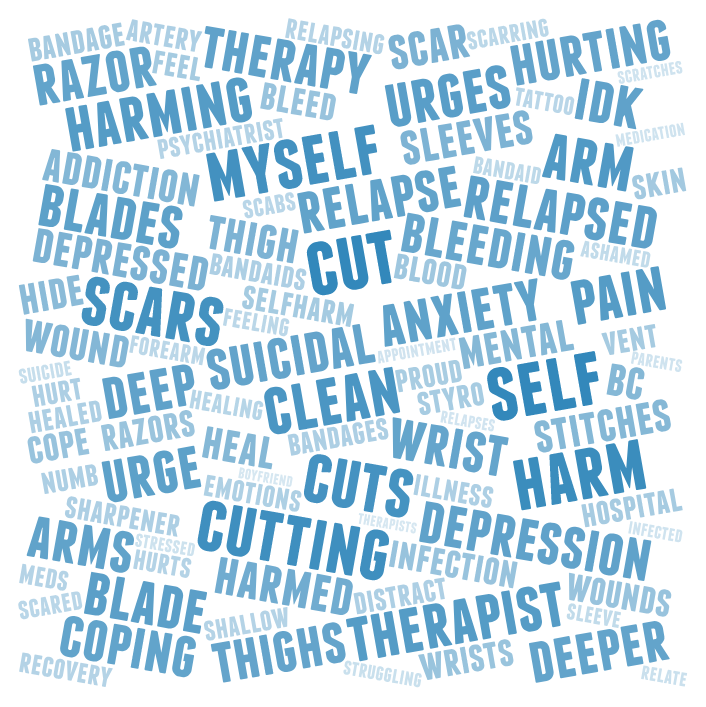
\includegraphics[width=\textwidth]{images/selfharm(gv)}
        \caption{Palabras}
        % \label{fig:word_cloud_a}
    \end{subfigure}
    \begin{subfigure}{0.5\textwidth}
        \centering
        
\includegraphics[width=\textwidth]{images/selfharm_bigrams(gv)}
        \caption{Bigramas}
        % \label{fig:word_cloud_b}
    \end{subfigure}
\caption{
    Top 100 palabras y bigramas seleccionados por el \emph{valor global} aprendido por, respectivamente, los modelos \emph{UNSL\#0} y \emph{UNSL\#1} de la tarea 2, detección de conductas autodestructivas.
    El tamaño de cada elemento se corresponde con su respectivo \emph{valor global}.
}
\label{fig:word_cloud_t2}
\end{figure*}

Al no contar con ningún tipo de conjunto de validación real, luego de que los modelos fueron entrenados, se los utilizó para generar una lista ordenada con los pares (palabra, \emph{valor global}) aprendidos por cada modelo.
A continuación, cada lista se revisó manualmente para corroborar que las palabras y valores aprendidos tuvieran cierto sentido en relación a la tarea sobre la que finalmente iban a ser evaluados.
Afortunadamente, a pesar de haber utilizado los mismos hiperparámetros en todos los modelos, las listas generadas coincidieron con lo esperado, como lo ilustran las nubes de palabras de la \autoref{fig:word_cloud_t2}.
Notar que este procedimiento de inspección manual fue posible gracias a que la transparencia y la simpleza formaron parte de los objetivos de diseño del modelo.\footnote{Ya que pocos son los modelos que permitirían, de forma simple y transparente, abordar preguntas tales como ``¿qué tan bien aprendió el modelo?¿qué tanto sentido tiene lo aprendido?'', sin la disponibilidad y el uso de un conjunto de validación sobre el que medir el desempeño.}


\vspace{5mm}

En relación a la tarea anterior, la efectividad general de todos los participantes fue menor en esta tarea.
Esto se debió a que, como se esperaba, la tarea representó un mayor reto para los modelos ya que, como se mencionó, no sólo no se proporcionaron datos de entrenamiento sino que la evidencia relacionada a las autolesiones podría ser muy escasa o, en muchos casos, incluso estar ausente ---ya que el conjunto de prueba no contó con ningún tipo de publicación creada luego de que los usuarios hayan decidido ingresar al foro de conductas autodestructivas.
% A continuación se presentarán los resultados obtenidos para esta tarea,
% Así, los principales resultados obtenidos con los 5 modelos descritos anteriormente, agrupados según las medidas utilizadas para medir el desempeño de los mismos, son los siguientes:
Los principales resultados obtenidos con los 5 modelos descritos anteriormente, agrupados según las medidas utilizadas para medir el desempeño de los mismos, son los siguientes:
% Los principales resultados globales obtenidos en esta tarea, tanto para las medidas centradas en la decisión como las basadas en ranking, se podrían resumir de la siguiente manera:


\begin{table*}[t!]
\centering
\caption{Resultados obtenidos en la tarea 2 para las medidas centradas en la decisión. A modo de comparación, del total de 29 modelos participantes, aquí se muestran, ordenados por $ERDE_{50}$, sólo los modelos que obtuvieron los mejores valores de cada uno de los otros 7 equipos de investigación.}
\label{tab:t2-result}
\begin{tabular}{l c c c c c}
\hline
Equipo\#modelo & $ERDE_5$ & $ERDE_{50}$ & $F_{latency}$ \\ \hline

UNSL\#0 & 9.01\% & 7.31\% & \textbf{.52} \\
UNSL\#1 & 9.03\% & 7.60\% & .50 \\
UNSL\#2 & 9.20\% & 6.86\% & .32 \\
UNSL\#3 & 8.79\% & 5.44\% & .45 \\
UNSL\#4 & \textbf{8.21\%} & \textbf{4.93\%} & .45 \\
\hline
\hline
BiTeM\#0 & 9.73\% & 7.63\% & .46 \\
BioInfo@UAVR\#0 & 10.79\% & 8.11\% & .45 \\
UDE\#2 & 13.75\% & 9.56\% & .28 \\
UDE\#1 & 11.27\% & 9.80\% & .29 \\
lirmm\#0 & 12.22\% & 10.02\% & .35 \\
CAMH\#4 & 14.84\% & 10.32\% & .22 \\
lirmm\#1 & 12.18\% & 10.58\% & .29 \\
LTL-INAOE\#2 & 12.53\% & 10.60\% & .22 \\
Fazl\#2 & 22.66\% & 13.23\% & .19 \\
Fazl\#1 & 22.66\% & 16.42\% & .18 \\
\hline

\end{tabular}
\end{table*}

\begin{itemize}
    % UNSL\#0 - Entre todos los participantes, este modelo obtuvo el mejor $F_{latency}$ ($.52$) y el mejor \emph{precision} ($.71$). Sin embargo, comparado con nuestros otros modelos, fue el que obtuvo el \emph{recall} más bajo ($.41$), junto con UNSL\#1 ($.39$), el cual también utilizó este mismo conjunto de datos.
    % UNSL\#2 - Este modelo obtuvo, de entre nuestros modelos, el mejor \emph{recall} ($.9$) pero los peores valores de \emph{precision} ($.2$) y $F_1$ ($.32$).
    % UNSL\#3 - Notablemente, el desempeño obtenido fue muy similar al del siguiente modelo, el cual obtuvo los mejores $ERDE_5$ y $ERDE_{50}$.

    

    \item \textbf{Desempeño centrado en la decisión:} en la \autoref{tab:t2-result} se muestran los resultados obtenidos para las medidas centradas en la decisión.
    En relación a las medidas $ERDE$ y $F_{latency}$, se puede observar que, de entre todos los participantes, el modelo \emph{UNSL\#4} obtuvo los mejores valores para $ERDE_5$ ($8.20\%$) y $ERDE_{50}$ ($4.93\%$), mientras que \emph{UNSL\#0} obtuvo el mejor valor $F_{latency}$ ($.52$). %\footnote{Además, si bien no se incluyen en esta tabla, este último también obtuvo los mejores \emph{precision} ($.71$) y $F_1$ ($.52$).}
    De entre los 5 modelos SS3, los dos entrenados con publicaciones individuales relacionadas a conductas autodestructivas, \emph{UNSL\#0 y \#1}, fueron los que mejor se desempeñaron en términos de la medida $F_{latency}$, pero los que obtuvieron el peor desempeñaron en términos de $ERDE_{50}$.
    Esto probablemente se haya debido a que estos modelos pudieron detectar con precisión a los usuarios cuya condición era más evidente (con publicaciones directamente vinculadas a conductas autodestructivas), pero dejando sin detectar a todos los otros usuarios en riesgo.\footnote{Esto también se vio reflejado en las medidas tradicionales, en donde \emph{UNSL\#0} obtuvo un $0.71$ de $precision$, pero un $0.41$ de $recall$.}
    Por lo tanto, dado que la medida de error $ERDE$ acumula más error cuando el modelo no detecta un caso en riesgo (falso negativo) que cuando detecta a uno que en realidad no lo era (falsos positivos), los errores $ERDE$ para estos modelos fueron mayores.
    Al igual que en la tarea anterior, y tal vez por los mismos motivos, el modelo $\tau$-SS3 (\emph{UNSL\#1}) obtuvo un desempeño ligeramente menor a su contraparte SS3 (\emph{UNSL\#0}) con este conjunto de datos.
    Por otro lado, el modelo \emph{UNSL\#2} fue el que obtuvo el peor desempeño de entre los 5 modelos, especialmente en las medidas $F_{latency}$ y $ERDE_5$, por lo que la incorporación de los tweets con hashtag ``\#selfharm'' al conjunto de entrenamiento produjo un impacto considerablemente negativo en el desempeño ---tal vez la información contenida en estos tweets aportó más ruido que información realmente útil para decidir si un usuario tiene conductas autodestructivas o no.
    En relación al modelo \emph{UNSL\#3}, entrenado con depresión y anorexia, obtuvo los segundos mejores valores $ERDE$ de entre todos los participantes, sólo por debajo del modelo \emph{UNSL\#4}, el cual también fue entrenado con depresión y anorexia pero ampliándolo con las publicaciones utilizadas para entrenar a los dos primeros modelos.
    Es importante resaltar que esto sugiere que, efectivamente, el vínculo con la depresión y la anorexia es lo suficientemente fuerte como para permitirle a SS3, en cierto grado, detectar usuarios padeciendo de conductas autodestructivas.
    Además, esto también podría sugerir que SS3 posee cierta robustez para lidiar con algunos escenarios de dominios cruzados.
    Esto último se ve reforzado por el hecho de que los modelos de UDE~\cite{masood2019ude} también fueron entrenados utilizando el mismo conjunto de entrenamiento que \emph{UNSL\#3}, anorexia y el depresión del eRisk 2018, y sin embargo, el desempeño de los mismos fue con diferencia más bajo que el de este último.
    Por ejemplo, \emph{UDE\#1} y \emph{UDE\#2} fueron los mismos modelos utilizados por UDE en la tarea anterior, estando el primero implementado con dos clasificadores SVM (uno utilizado para filtrar publicaciones no relevantes y otro para tomar la decisión final) y estando el segundo implementado con una red neuronal recurrente LSTM tomando como entrada un vector \emph{doc2vec} representando las publicaciones leídas hasta el momento.
    Sin embargo, \emph{UDE\#1} obtuvo un $ERDE_{50}$ de $9.80\%$ y un $F_{latency}$ de $0.29$, y \emph{UDE\#2} un $ERDE_{50}$ de $9.56\%$ y un $F_{latency}$ de $0.28$, mientras que \emph{UNSL\#3} obtuvo un error $ERDE_{50}$ considerablemente menor ($5.44\%$) y un $F_{latency}$ considerablemente mayor ($0.45$), habiendo sido entrenado con los mismos datos ---sugiriendo que SS3 se adaptó considerablemente mejor al cambio de dominio que los dos primeros, los cuales se (sobre)ajustaron al dominio original en el que fueron entrenados (anorexia y depresión).
    Como se verá luego en el \autoref{cap:conclusion}, este aspecto no es secundario y será considerado como línea de trabajo a ser explorada como trabajo a futuro.

\begin{table*}[t!]
\centering
\caption{Detalle de los equipos participantes en la tarea 2: nombre del equipo, cantidad de modelos empleados ($\#modelos$), número de publicaciones procesadas de los usuarios ($\#publicaciones$), tiempo total empleado para completar la tarea y tiempo empleado para procesar cada publicación (\emph{i.e.} $\frac{tiempo\ total}{\#publicaciones\times\#modelos}$).}%Participating teams for Task 2: number of runs, number of user writings processed by the team, and the time taken for the whole process and for processing each writing (i.e $\frac{TotalTime}{\#writings\times\#runs}$). (*) This value was originally 5, but we replaced it by the actual number of models used.
\label{tab:t2-time}
\begin{tabular}{l c c|c | c}
\hline
& & & \multicolumn{2}{c}{Tiempo} \\
Equipo & \#modelos & \#publicaciones & total & por publicación  \\ \hline

\textbf{UNSL}$\star$ & 5 & 1992 & 13h & \textbf{4.6s} \\
BioInfo@UAVR & 1 & 1992 & 4h & 7.2s \\
LTL-INAOE & 4 & 1993 & 17h & 7.6s \\
BiTeM & 2 & 8 & 3m & 11.2s \\
UDE & 4 & 1992 & 1 día + 2h & 11.7s \\
CAMH & 5 & 1992 & 1 día + 19h & 15.5s \\
lirmm & 5 & 2004 & 2 días + 22h & 25.1s \\
Fazl & 3 & 1993 & 18 días + 21h & 4m + 32s \\

\hline
\end{tabular}
\end{table*}

    \item \textbf{Desempeño en relación al tiempo de ejecución:} en la \autoref{tab:t2-time} se muestran, por cada equipo, detalles sobre el tiempo total empleado para completar la tarea.
    Como se puede observar, a diferencia de la primer tarea, el tiempo empleado fue relativamente similar entre cada equipo, siendo Fazl la única excepción, habiéndole tomado 18 días y 21 horas completar la tarea.
    Nuevamente se puede observar que UNSL fue, aunque no por mucho, el equipo más eficiente en términos de tiempos de ejecución ya que procesó las 1992 publicaciones de cada usuario con cada uno de los 5 modelos en 13 horas, por lo que cada modelo procesó cada publicación en aproximadamente 4.6 segundos.
    % como se muestra en la \autoref{tab:t2-time}, en esta tarea también fuimos los más rápidos en procesar las publicaciones, procesando cada una en poco menos de 5 segundos, tomándonos 13 horas en total completar la tarea.
    % Notar que si bien a simple vista puede parecer que BioInfo@UAVR~\cite{trifan2019bioinfo} fue más rápido, al completar la tarea en 4 horas, también se debe tener en cuenta que tuvo que procesar y enviar 5 veces menos publicaciones y respuestas al servidor que nosotros ---ya que participaron con un único modelo.

\begin{table*}[t!]
\centering
\caption{Resultados obtenidos en la tarea 2 para las medidas basadas en ranking para 4 rankings distintos, respectivamente, el ranking obtenido luego de leer 1, 100, 500 y 1000 publicaciones. Aquí también se incluyen, a modo de comparación, los mejores resultados obtenidos por los otros 7 equipos.}
\label{tab:t2-result-ranking}
\begin{tabular}{l c c c|c c c}
\hline
& \multicolumn{3}{c}{1 publicación leída} & \multicolumn{3}{c}{100 publicaciones leídas} \\
Equipo\#modelo & P@10 & NDCG@10 & NDCG@100 &  P@10 & NDCG@10 & NDCG@100 \\ \hline

UNSL\#0 & .7 & .79 & .48 & \textbf{.9} & \textbf{.94} & .61 \\
UNSL\#1 & .6 & .74 & .48 & \textbf{.9} & \textbf{.94} & .60 \\
UNSL\#2 & .9 & .88 & .62 & .8 & .75 & .75 \\
UNSL\#3 & \textbf{1} & \textbf{1} & \textbf{.67} & \textbf{.9} & \textbf{.94} & .84 \\
UNSL\#4 & \textbf{1} & \textbf{1} & .64 & \textbf{.9} & .93 & \textbf{.86} \\
\hline\hline
Fazl\#1 & .2 & .27 & .36 & \textbf{.9} & \textbf{.94} & .83 \\
CAMH\#0 & .3 & .37 & .47 & .6 & .71 & .49 \\
UDE\#1 & .7 & .56 & .52 & .7 & .66 & .69 \\
CAMH\#2 & .3 & .41 & .51 & .5 & .62 & .39 \\
UDE\#2 & .5 & .63 & .53 & .5 & .56 & .64 \\
LTL-INAOE\#0 & .5 & .5 & .45 & .4 & .41 & .55 \\
LTL-INAOE\#1 & .6 & .73 & .56 & .1 & .19 & .17 \\
BiTeM\#4 & .4 & .56 & .50 & - & - & - \\
BiTeM\#2 & .5 & .48 & .44 & - & - & - \\
BiTeM\#0 & .3 & .35 & .53 & - & - & - \\
lirmm\#0 & .1 & .19 & .15 & 0 & 0 & .01 \\


\hline
\hline
\end{tabular}

\

\

\begin{tabular}{l c c c|c c c}
\hline
& \multicolumn{3}{c}{500 publicaciones leídas} & \multicolumn{3}{c}{1000 publicaciones leídas} \\
Equipo\#modelo & P@10 & NDCG@10 & NDCG@100 &  P@10 & NDCG@10 & NDCG@100 \\ \hline

UNSL\#0 & \textbf{.9} & \textbf{.94} & .66 & \textbf{.9} & \textbf{.94} & .66 \\
UNSL\#1 & \textbf{.9} & \textbf{.94} & .65 & \textbf{.9} & \textbf{.94} & .65 \\
UNSL\#2 & .5 & .59 & .74 & .6 & .64 & .74 \\
UNSL\#3 & .7 & .63 & .75 & .7 & .63 & .75 \\
UNSL\#4 & .7 & .67 & \emph{.79} & .8 & .74 & \emph{.78} \\
\hline\hline
Fazl\#1 & \textbf{.9} & \textbf{.94} & \textbf{.84} & \textbf{.9} & \textbf{.94} & \textbf{.84} \\
UDE\#1 & .8 & .75 & .74 & .8 & .75 & .74 \\
CAMH\#0 & .7 & .72 & .50 & .6 & .66 & .48 \\
CAMH\#2 & .7 & .72 & .45 & .6 & .66 & .44 \\
UDE\#2 & .6 & .66 & .68 & .6 & .65 & .67 \\
LTL-INAOE\#0 & .2 & .19 & .25 & .1 & .19 & .37 \\
LTL-INAOE\#1 & .1 & .06 & .07 & 0 & 0 & .04 \\

\hline
\hline
\end{tabular}

\end{table*}

    \item \textbf{Desempeño basado en ranking:} en la \autoref{tab:t2-result-ranking} se muestran los resultados obtenidos para las medidas basadas en ranking.
    Se puede observar que, si bien hubo una caída general en el desempeño de los modelos SS3 en relación a los obtenidos en la primer tarea, nuevamente se obtuvieron los mejores valores para las medidas $P@10$ y $NDCG@10$ en los 4 rankings y los mejores valores en la medida $NDCG@100$ para los rankings obtenidos luego de procesar $1$ y $100$ publicaciones, y el segundo mejor luego de procesar $500$ y $1000$ publicaciones.
    En relación al desempeño de las distintas variantes utilizadas, la principal diferencia se encuentra entre los modelos entrenados con publicaciones individuales (\emph{UNSL\#0 y \#1}) y los entrenados con depresión y anorexia (\emph{UNSL\#3 y \#4}), siendo los primeros mejores en términos de $P@10$ y $NDCG@10$, y los segundos en términos de $NDCG@100$.
    Esto posiblemente se deba a los mismos motivos expuestos anteriormente en relación al desempeño basado en decisión, en donde los primeros obtuvieron el mejor $F_{latency}$ y los segundos los mejores valores $ERDE$.\footnote{Los primeros son más precisos en detectar usuarios con mayor evidencia explícita, pero, a diferencia de los segundos, dejan a gran parte de los usuarios en riesgo sin detectar, pudiendo así armar un ranking de 10 usuarios pero fallando en armar un ranking mayor, de 100 usuarios, en donde todos los 61 usuarios en riesgo deberían estar presentes.}
    Finalmente, en relación al modelo entrenado con tweets, \emph{UNSL\#2}, al igual que con las medidas basadas en decisión, su desempeño fue el peor de entre los 5 modelos ---no obtuvo un mejor valor en ninguna medida y en ningún ranking.
    En líneas generales, es interesante notar que pese a haber sido entrenados con distintos conjuntos de datos, incluido datos de otros dominios, los modelos SS3 obtuvieron resultados consistentemente buenos en relación a los otros modelos, y más importante aún, a lo largo de los distintos tipos de medidas de desempeño utilizadas.
    Esto contrasta con otros modelos que si bien se desempeñaron bien en relación a ciertos aspectos de la problemática abordada, no lo hicieron robusta y consistentemente en relación a otros.
    Por ejemplo, el modelo \emph{Fazl\#1} obtuvo un buen desempeño en las medidas de ranking, obteniendo el mejor valor $NDCG@100$ para los rankings generados luego de leer 500 y 1000 publicaciones, sin embargo, como se observó en la \autoref{tab:t1-result}, obtuvo el peor desempeño de entre todos los modelos participantes en relación a las medidas centradas en la decisión, a pesar de haber demorado cerca de 19 días en completar la tarea.
    Finalmente, notar que al igual que en la tarea anterior, SS3 parece ser capaz de estimar el nivel de riesgo de los usuarios, con cierta eficiencia, aún cuando muy poca información ha sido procesada.
    Por ejemplo, como se observa en la sección ``1 publicación leída'' de la \autoref{tab:t2-result-ranking},
    todos los modelos obtuvieron mejores resultados que el resto de los modelos, a pesar de haber sido entrenados con distintos datos.
    Además, en relación a este último punto, es interesante destacar el hecho que los modelos \emph{UNSL\#3 y \#4} hayan sido capaces de construir un ranking ideal de 10 usuarios en riesgo (\emph{i.e.} $NDCG@10 = 1$) habiendo leído solamente la primer publicación de cada usuario.


\end{itemize}



% \subsection{Tarea 3: Medición de la Gravedad de la Depresión}%Task 3: Measuring the severity of the signs of depression

% participaron 8 equipos.

% %This task was really difficult since it was not a single ``yes or no'' problem but a problem involving multiple decisions, one for each one of the 21 questions. To make things even harder, as with Task 2, no training data was released either.
% Esta tarea fue realmente difícil ya que no se trataba de un solo problema de `` sí o no '' sino de un problema que involucraba múltiples decisiones, una para cada una de las 21 preguntas. Para hacer las cosas aún más difíciles, como con la Tarea 2, tampoco se publicaron datos de entrenamiento.
% %Fortunately, early depression detection is a task we had some previous experience working with since we had participated in the two previous eRisk labs (2017\cite{burdisso2019} and 2018\cite{funez2018}).
% Afortunadamente, la detección temprana de la depresión es una tarea con la que teníamos experiencia previa trabajando desde que habíamos participado en los dos laboratorios de eRisk anteriores (2017\cite{burdisso2019} y 2018\cite{funez2018}).
% %Therefore, we decided to train SS3 using the dataset for the eRisk 2018 depression detection task.
% Por lo tanto, decidimos entrenar SS3 utilizando el conjunto de datos para la tarea de detección de depresión eRisk 2018.
% %However, the main problem was deciding how to turn this ``yes or no'' classifier into a classifier capable of filling BDI questionnaires. We came up with the idea of using the \emph{confidence vector}, $\overrightarrow{d}$ in  \autoref{eq:sum_gv}, to somehow infer a BDI depression level between 0 and 63. To achieve this, first, we converted the \emph{confidence vector} into a single \emph{confidence value} normalized between 0 and 1, by applying the following equation:
% Sin embargo, el principal problema fue decidir cómo convertir este clasificador de `` sí o no '' en un clasificador capaz de llenar cuestionarios BDI. Se nos ocurrió la idea de usar el \emph{vector de confianza}, $\overrightarrow{d}$ en \autoref{eq:sum_gv}, para inferir de alguna manera un nivel de depresión del BDI entre 0 y 63. Para lograr esto, primero convertimos el \emph{vector de confianza} en un \emph{valor de confianza} único normalizado entre 0 y 1, aplicando la siguiente ecuación:

% \begin{equation}
%     confidence\_value = \frac{d[positive]-d[negative]}{d[positive]}
%     \label{eq:conf_val}
% \end{equation}

% % \begin{equation}
% %     depression\_level = \frac{d[positive]-d[negative]}{d[positive]}\times63
% % \end{equation}

% %Then, after SS3 classified a subject, the obtained $confidence\_value$ was divided into 4 regions, one for each BDI depression category. This was carried out by the following equation:
% Luego, después de que SS3 clasificara a un sujeto, la $confidence\_value$ obtenida se dividió en 4 regiones, una para cada categoría de depresión del BDI. Esto se llevó a cabo mediante la siguiente ecuación:

% \begin{equation}
%     c = \lfloor confidence\_value \times 4\rfloor
%     \label{eq:c}
% \end{equation}

% %And finally, the subject depression level was predicted by mapping the percentage of $confidence\_value$ left inside the predicted $c$ region to its corresponding BDI depression level range (e.g. $(0.5, 0.75]\longrightarrow[19,29]$ for $c = 2 =$ ``moderate depression'') by computing the following:
% Y finalmente, el nivel de depresión del sujeto se predijo mapeando el porcentaje de $confidence\_value$ que queda dentro de la región $c$ predicha a su rango de nivel de depresión BDI correspondiente (por ejemplo, $(0.5, 0.75]\longrightarrow[19,29]$ para $c = 2 =$ ``depresión moderada'') calculando lo siguiente:

% \begin{equation}
%     depression\_level = min_c + \lfloor(max_c - min_c + 1) \times (confidence\_value \times 4 - c)\rfloor
%     \label{eq:dep_lvl}
% \end{equation}
% %Where $min_c$ and $max_c$ are the lower and upper bound for category $c$,  respectively (e.g. 19 and 29 for ``moderate depression'' category). 
% Donde $min_c$ y $max_c$ son el límite inferior y superior para la categoría $c$, respectivamente (por ejemplo, 19 y 29 para la categoría de `` depresión moderada '').


% \begin{figure}[t!] % [t]op; [h]ere; [p]age; [b]ottom; [r]ight; [l]eft
%     \centering
%     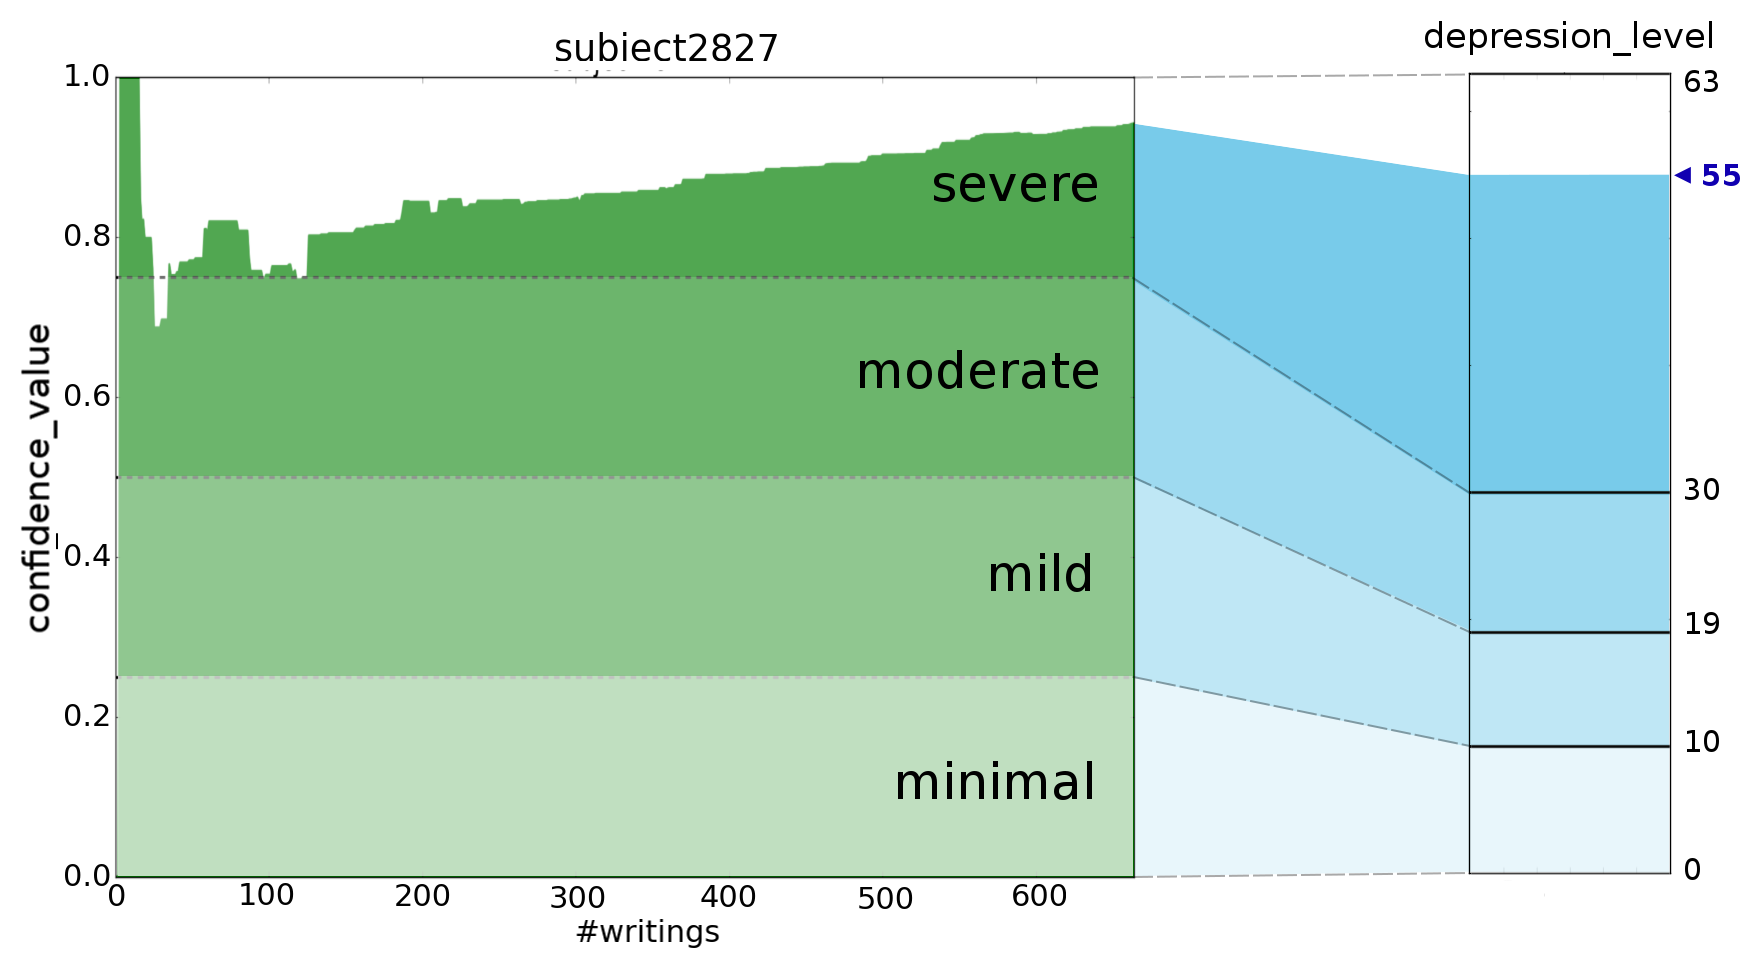
\includegraphics[width=120mm]{images/subject2827-bdi}
%     \caption{Diagrama del proceso de cálculo de \emph{depression\_level} para el sujeto 2827. Como puede notar el lector, después de procesar todos los escritos del sujeto, el \emph{confidence\_value} (0,941) final se mapeó en su \emph{depression\_level} (55) correspondiente.}%Diagram of the \emph{depression\_level} computation process for subject 2827. As reader can notice, after processing all the subject's writings, the final \emph{confidence\_value} (0.941) was mapped into its corresponding \emph{depression\_level} (55).
%     \label{fig:subject-bdi}
% \end{figure}

% \vspace{5mm}

% \begin{figure*}[t!]
%     \begin{subfigure}{0.5\textwidth}
%         \centering
%         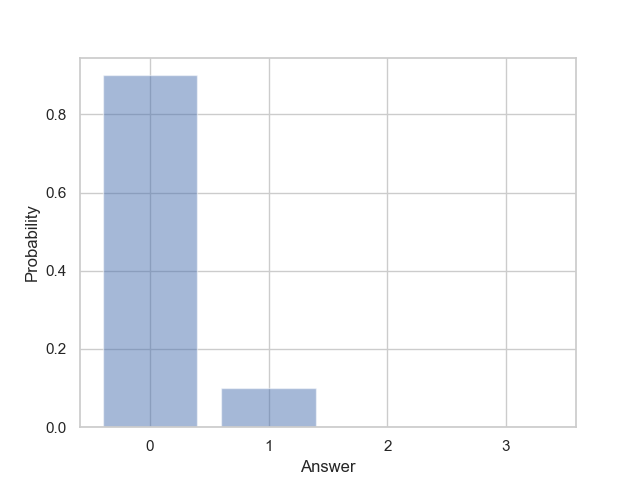
\includegraphics[width=65mm]{images/distp-exp0.png}
%         \caption{If expected answer is 0}
%     \end{subfigure}
%     \begin{subfigure}{0.5\textwidth}
%         \centering
%         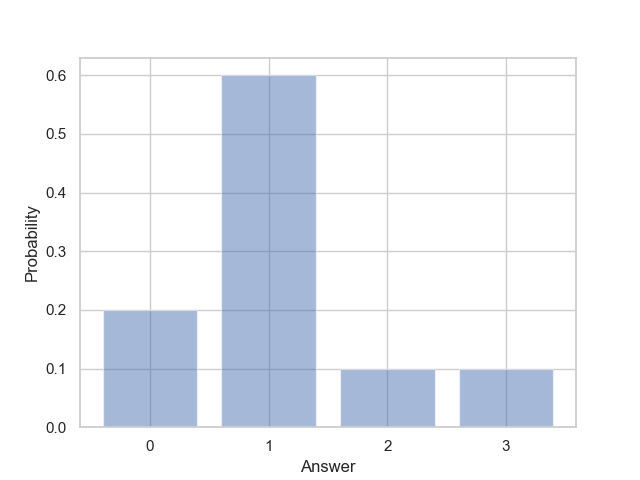
\includegraphics[width=65mm]{images/distp-exp1.png}
%         \caption{If expected answer is 1}
%     \end{subfigure}
%     \begin{subfigure}{0.5\textwidth}
%         \centering
%         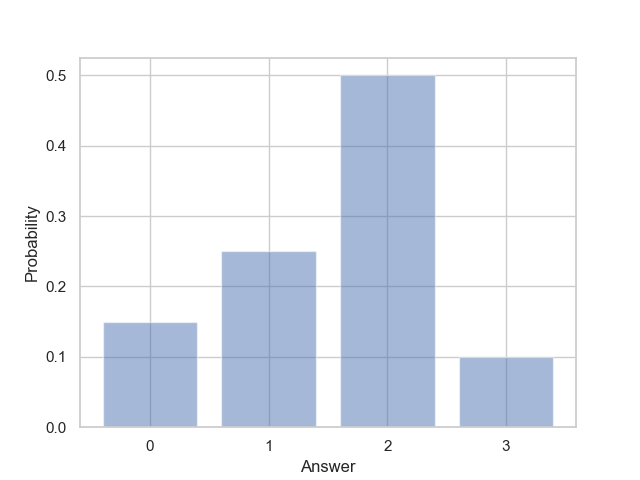
\includegraphics[width=65mm]{images/distp-exp2.png}
%         \caption{If expected answer is 2}
%     \end{subfigure}
%     \begin{subfigure}{0.5\textwidth}
%         \centering
%         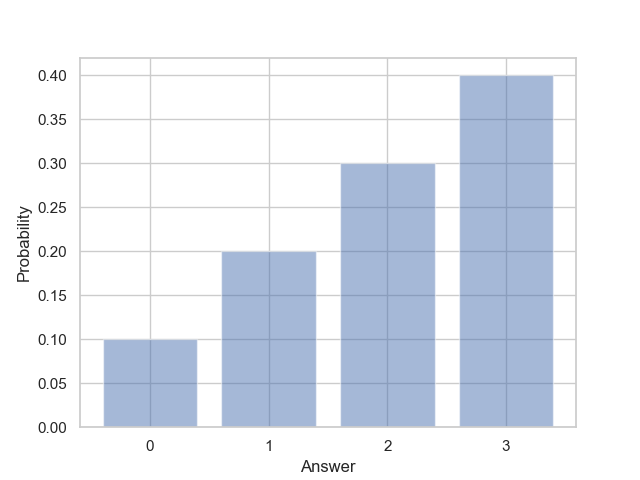
\includegraphics[width=65mm]{images/distp-exp3.png}
%         \caption{If expected answer is 3}
%     \end{subfigure}
% \caption{
%     Distribución de probabilidad discreta para cada posible respuesta esperada.
% }%Discrete probability distribution for each possible expected answer.
% \label{fig:distprob-t3}
% \end{figure*} 

% %In order to clarify the above process, we will illustrate it with the example shown in \autoref{fig:subject-bdi}. First, SS3 processed the entire writing history computing the $confidence\_value$ (given by \autoref{eq:conf_val}) and then, the final $confidence\_value$ (0.941) was used to predict the depression category, ``severe depression'' ($c = 3$), by using the \autoref{eq:c}. Finally, the depression level was computed by the mapping given by \autoref{eq:dep_lvl}, as follows:
% Para aclarar el proceso anterior, lo ilustraremos con el ejemplo que se muestra en \autoref{fig:subject-bdi}. Primero, SS3 procesó todo el historial de escritura calculando el $confidence\_value$ (dada por \autoref{eq:conf_val}) y luego, el $confidence\_value$ final (0.941) se usó para predecir la categoría de depresión, `` depresión severa '' ($c = 3$), usando la \autoref{eq:c}. Finalmente, el nivel de depresión se calculó mediante el mapeo proporcionado por \autoref{eq:dep_lvl}, de la siguiente manera:

% \begin{equation}
%     \begin{split}
%     depression\_level & = 30 + \lfloor(63 - 30 + 1) \times (0.941\times4 - 3)\rfloor \\
%     & = 
%     30 + \lfloor34 \times (3.764 - 3)\rfloor = 30 + \lfloor34 \times 0.764\rfloor \\
%     & = 30 + 25 = \textbf{55}
%     \end{split}
% \end{equation}



% %At this point, we have transformed the output of SS3 from a 2-dimensional vector, $d$, into a BDI depression level (a value between 0 and 63).
% En este punto, hemos transformado la salida de SS3 de un vector bidimensional, $d$, a un nivel de depresión BDI (un valor entre 0 y 63).
% %However, we have not covered yet how to actually answer the 21 questions in the BDI questionnaire using this \emph{depression level}.
% Sin embargo, todavía no hemos cubierto cómo responder realmente a las 21 preguntas del cuestionario BDI utilizando este \emph{nivel de depresión}.
% %Regardless of the method, we decided that for all those users whose $depression\_level$ was less or equal to 0, all the BDI questions were answered with 0. For the other users we applied different methods, depending on the run, as described below:
% Independientemente del método, decidimos que para todos aquellos usuarios cuyo $depression\_level$ fuera menor o igual a 0, todas las preguntas de BDI se respondieran con 0. Para los demás usuarios aplicamos diferentes métodos, según la ejecución, como se describe a continuación:

% \begin{itemize}
%     %\item \emph{UNSLA}: using the predicted \emph{depression\_level} our model filled the questionnaires answering the expected number ($\lfloor\frac{depression\_level}{21}\rfloor$) on each question. If this division had a remainder, the remainder points were randomly scattered so that the sum of all the answers always matched the predicted depression level given by SS3.
%     \item \emph{UNSLA}: utilizando el \emph{depression\_level} predicho, nuestro modelo llenó los cuestionarios respondiendo el número esperado ($\lfloor\frac{depression\_level}{21}\rfloor$) en cada pregunta. Si esta división tenía un resto, los puntos restantes se dispersaron aleatoriamente para que la suma de todas las respuestas siempre coincidiera con el nivel de depresión predicho dado por SS3.
%     %\item \emph{UNSLB}: this time, only the predicted category, $c$, was used. Our model filled the questionnaire randomly in such a way that the final depression level always matched the predicted category. Compared to the following three ones, these two models were the ones with the worst performance.
%     \item \emph{UNSLB}: esta vez, sólo se utilizó la categoría predicha, $c$. Nuestro modelo llenó el cuestionario al azar de tal manera que el nivel de depresión final siempre coincidió con la categoría prevista. En comparación con los siguientes tres, estos dos modelos fueron los que presentaron el peor rendimiento.
%     %\item \emph{UNSLC}: this model and the followings were more question-centered.
%     \item \emph{UNSLC}: este modelo y los siguientes estaban más centrados en preguntas.
%     %Once again, as in UNSLA, our model filled the questionnaires answering the expected number derived from the predicted depression level ($\lfloor\frac{depression\_level}{21}\rfloor$). But this time, answering this number only on questions for which a ``textual hint'' for a possible answer was found in the user's writings, and randomly and uniformly answered between 0 and $\ceil[big]{\frac{depression\_level}{21}}$ otherwise. To find this ``textual hint'', our model split the user's writings into sentences and searched for the co-occurrence of the word ``I'' or ``my'' with at least one word matching a regular expression specially crafted for each question.\footnote{e.g. ``(sad)$|$(unhappy)'' for question 1, ``(future)$|$(work out)'' for question 2, ``fail\textbackslash w*'' for question 3, ``(pleasure)$|$(enjoy)'' for question 4, etc. } This method obtained the best AHR (41.43\%) and the second-best DCHR (40\%).
%     Una vez más, como en UNSLA, nuestro modelo llenó los cuestionarios respondiendo el número esperado derivado del nivel de depresión pronosticado ($\lfloor\frac{depression\_level}{21}\rfloor$). Pero esta vez, respondiendo a este número solo en preguntas para las que se encontró una ``pista textual'' para una posible respuesta en los escritos del usuario, y se respondió de manera aleatoria y uniforme entre 0 y $\ceil[big]{\frac{depression\_level}{21}}$ en caso contrario. Para encontrar esta ``pista textual'', nuestro modelo dividió los escritos del usuario en oraciones y buscó la co-ocurrencia de la palabra ``I'' o ``my'' con al menos una palabra que coincida con una expresión regular especialmente diseñada para cada pregunta.\footnote{p.ej. ``(triste)$|$(infeliz)'' para la pregunta 1, ``(futuro)$|$(resolver)'' para la pregunta 2, ``fail\textbackslash w*'' para la pregunta 3, ``(placer)$|$(disfrutar)'' para la pregunta 4, etc.} Este método obtuvo el mejor AHR (41,43\%) y el segundo mejor DCHR (40\%).
    
%     %\item \emph{UNSLD}: the same as the previous one, but not using the ``textual hints'',  i.e. always answering every question randomly and uniformly between 0 and $\ceil[big]{\frac{depression\_level}{21}}$. This model was mainly used only with the goal of measuring the actual impact of using these ``textual hints'' to decide which questions should be answered with the expected answer ($\lfloor\frac{depression\_level}{21}\rfloor$).
%     \item \emph{UNSLD}: el mismo que el anterior, pero sin utilizar las ``pistas textuales'', es decir, siempre respondiendo todas las preguntas de forma aleatoria y uniforme entre 0 y $\ceil[big]{\frac{depression\_level}{21}}$. Este modelo se utilizó principalmente solo con el objetivo de medir el impacto real de utilizar estas ''sugerencias textuales'' para decidir qué preguntas deben responderse con la respuesta esperada (F$\lfloor\frac{depression\_level}{21}\rfloor$).
%     %\item \emph{UNSLE}: the same as UNSLD, but this time not using a uniform distribution. More precisely, from the overall depression level predicted by SS3, once again the expected answer was computed ($\lfloor\frac{depression\_level}{21}\rfloor$) and, depending on the value of the expected answer, actual answers were given following the probability distributions shown in \autoref{fig:distprob-t3}. Note that, unlike uniform distribution (used in UNSLD), when using these probability distributions the expected answer is more likely to be selected over the other ones. This model obtained the best ACR (71.27\%) and the second-best AHR (40.71\%) and ADODL (80.48\%, best was only 0.54\% above).
%     \item \emph{UNSLE}: lo mismo que UNSLD, pero esta vez sin utilizar una distribución uniforme. Más precisamente, a partir del nivel de depresión general predicho por SS3, una vez más se calculó la respuesta esperada ($\lfloor\frac{depression\_level}{21}\rfloor$) y, dependiendo del valor de la respuesta esperada, las respuestas reales se dieron siguiendo las distribuciones de probabilidad mostradas en \autoref{fig:distprob-t3}. Tenga en cuenta que, a diferencia de la distribución uniforme (utilizada en UNSLD), cuando se utilizan estas distribuciones de probabilidad, es más probable que se seleccione la respuesta esperada sobre las otras. Este modelo obtuvo el mejor ACR (71,27\%) y el segundo mejor AHR (40,71\%) y ADODL (80,48\%, el mejor fue solo un 0,54\% por encima).
% \end{itemize}

% \begin{table*}[t!]
% \centering
% \caption{Resultados de la tarea T3. para referencia, al final se ha añadido el promedio de completar el formulario al azar 1000 veces. }
% \label{tab:t3-result}
% \begin{tabular}{l c c c c}
% \hline
% Modelo & AHR & ACR & ADODL & DCHR \\ \hline

% UNSLA & 37.38\% & 67.94\% & 72.86\% & 30\% \\
% UNSLB & 36.93\% & 70.16\% & 76.83\% & 30\% \\
% UNSLC & \textbf{41.43\%} & 69.13\% & 78.02\% & \emph{40\%} \\
% UNSLD & 38.10\% & 67.22\% & 78.02\% & 30\% \\
% UNSLE & 40.71\% & \textbf{71.27\%} & \emph{80.48\%} & 35\% \\
% CAMH unsupervised & 23.81\% & 57.06\% & \textbf{81.03\%} & \textbf{45\%} \\
% CAMH supervised (SVM - LIWC) & 35.95\% & 66.59\% & 75.48\% & 25\% \\
% CAMH supervised (GPT - 180 features) & 35.47\% & 68.33\% & 75.63\% & 20\% \\
% CAMH supervised (GPT - 768 features) & 36.43\% & 67.22\% & 72.30\% & 20\% \\
% CAMH supervised (GPT - 948 features) & 36.91\% & 69.13\% & 75.63\% & 15\% \\
% BioInfo@UAVR & 34.05\% & 66.43\% & 77.70\% & 25\% \\
% BiTeM & 32.14\% & 62.62\% & 72.62\% & 25\% \\
% Fazl & 22.38\% & 56.27\% & 72.78\% & 5\% \\
% Illinois & 22.62\% & 56.19\% & 66.35\% & 40\% \\
% ISIKol multiSimilarity-5000-Dtac-Qtac & 29.76\% & 57.94\% & 74.13\% & 25\% \\
% ISIKol-bm25-1.2-0.75-5000-Dtac-Qtac & 29.76\% & 57.06\% & 72.78\% & 25\% \\
% ISIKol-lm-d-1.0-5000-Dtac-Qtac & 30.00\% & 57.94\% & 73.02\% & 15\% \\
% Kimberly & 38.33\% & 64.44\% & 66.19\% & 20\% \\
% \hline
% \hline
% Al Azar (promedio de 1000 repeticiones) & 23.98\% & 58.55\% & 77.78\% & 33.55\% \\
% \hline
% \end{tabular}
% \end{table*}

% \begin{table*}[t!]
% \centering
% \caption{Resultados de la Tarea 3. Ahora los resultados de nuestras ejecuciones se muestran utilizando un intervalo de confianza del 95\%.}%Results for Task 3. Now our runs results are shown using a 95\% confidence interval.
% \label{tab:t3-result-mean}
% \centerline{
% \begin{tabular}{l c c c c}
% \hline
% Modelo & AHR & ACR & ADODL & DCHR \\ \hline

% %CAMH\_GPT\_nearest\_unsupervised & 23.81\% & 57.06\% & 81.03\% & \textbf{45\%} \\
% UNSLA & 38.13\% $\pm$ 2.29\% & 68.30\% $\pm$ 0.84\% & 72.62\% & 30\% \\
% UNSLB & 38.97\% $\pm$ 2.65\% & \textbf{69.77\% $\pm$ 1.98\%} & 74.72\% $\pm$ 2.82\% & 30\% \\
% UNSLC & \textbf{40.19\% $\pm$ 3.14\%} & 69.26\% $\pm$ 1.75\% & 77.53\% $\pm$ 1.92\% & 29.91\% $\pm$ 8.70\% \\
% UNSLD & 39.26\% $\pm$ 3.21\% & 68.72\% $\pm$ 1.81\% & 77.56\% $\pm$ 1.86\% & 30.86\% $\pm$ 11.14\% \\
% UNSLE & 38.18\% $\pm$ 3.41\% & 69.61\% $\pm$ 1.95\% & \textbf{82.94\% $\pm$ 2.17\%} & \textbf{38.42\% $\pm$ 10.14\%} \\
% \hline
% \end{tabular}}
% \end{table*}

% % \begin{figure*}[t!]
% %     \begin{subfigure}{0.5\textwidth}
% %         \centering
% %         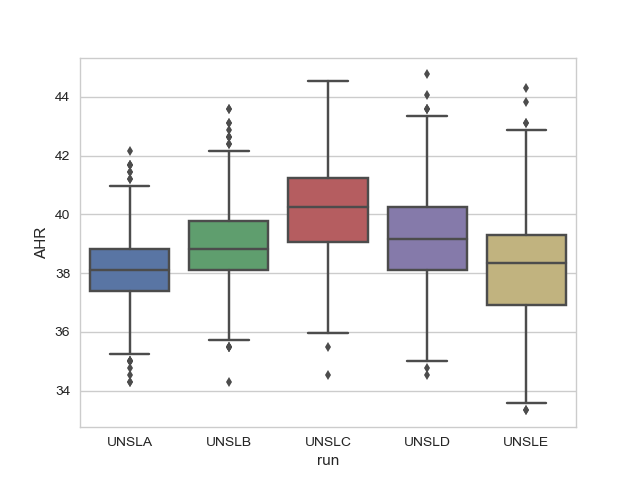
\includegraphics[width=68.5mm]{images/AHR}
% %         \caption{AHR}
% %         \label{fig:plot-result-t3-ahr}
% %     \end{subfigure}
% %     \begin{subfigure}{0.5\textwidth}
% %         \centering
% %         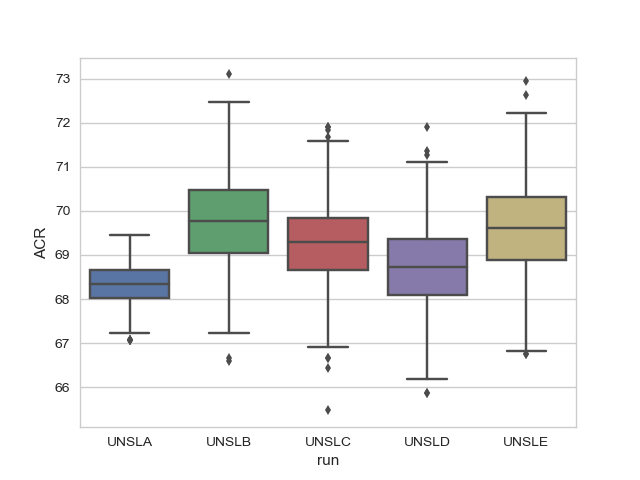
\includegraphics[width=68.5mm]{images/ACR}
% %         \caption{ACR}
% %     \end{subfigure}
% %     \begin{subfigure}{0.5\textwidth}
% %         \centering
% %         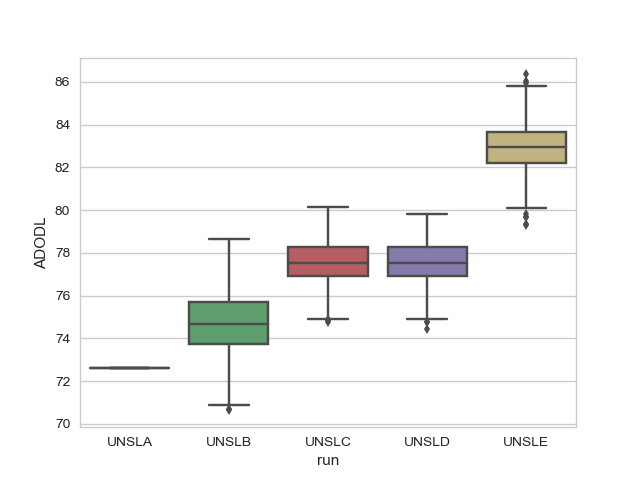
\includegraphics[width=68.5mm]{images/ADODL}
% %         \caption{ADODL}
% %         \label{fig:plot-result-t3-adodl}
% %     \end{subfigure}
% %     \begin{subfigure}{0.5\textwidth}
% %         \centering
% %         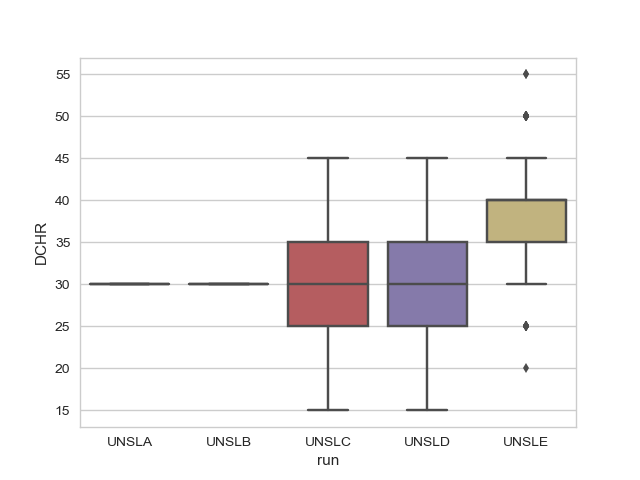
\includegraphics[width=68.5mm]{images/DCHR}
% %         \caption{DCHR}
% %     \end{subfigure}
% % \caption{
% %     Box plots for each measure and run.
% % }
% % \label{fig:plot-result-t3}
% % \end{figure*} 

% %The obtained results are shown in \autoref{tab:t3-result}. As mentioned above, we obtained the best AHR (41.43\%) and ACR (71.27\%), and the second-best ADODL (80.48\%) and DCHR (40\%). However, since most of our models' answers are randomly generated, it implies that all of these measures are also stochastically generated.\footnote{Only ADODL and DCHR for UNSLA and 
% Los resultados obtenidos se muestran en \autoref{tab:t3-result}. Como se mencionó anteriormente, obtuvimos el mejor AHR (41.43\%) y ACR (71.27\%), y el segundo mejor ADODL (80.48\%) y DCHR (40\%). Sin embargo, dado que la mayoría de las respuestas de nuestros modelos se generan aleatoriamente, esto implica que todas estas medidas también se generan estocásticamente.\footnote{Solo ADODL y DCHR para UNSLA y 
% %DHR for UNSLB are deterministically determined by $depression_level$ and $c$.} The natural question in cases like this is ``How do we know these results properly represent our models' performance and we did not obtain them just by pure chance?''. In order to clarify this, we run each model 1000 times and calculated the values for AHR, ACR, ADODL and DCHR each time\footnote{Just as if we had participated 1000 times in this task.}. After this process finished, we ended up with a sample of 1000 values for each measure and model, which we then used to produce the results shown in \autoref{tab:t3-result-mean}. Results have been replaced by intervals with 95\% of confidence, which better represent our performance. One can notice that, in fact, when we participated we had a little bit of bad luck, especially for UNSLE's ADODL, because the actual value we obtained (80.84\%) is almost a lower bound outlier. Another thing that we can notice, comparing UNSLC and UNSLD, is that the use of ``textual hints'' slightly improves the Average Hit Rate (AHR) but does not impact on the other measures. UNSLE is considerably the best method to estimate the overall depression level since it takes values within a range that is quite above the others. Additionally, another important point is that taking into account these 95\% confidence intervals, the obtained values would be among the best ones even in the worst cases. Finally, since all the methods we used are based on the depression level predicted by SS3, this shows us that SS3 is correctly inferring the depression level from the textual evidence accumulated while processing the user's writings, i.e. SS3 is correctly valuing words in relation to each category (depressed and non-depressed) which is consistent with the results obtained for the ranking-based measures for task T1 and T2. Additionally, this could also imply that could really be a relationship between how subjects write (what words they use) and the actual depression level they have.
% DHR para UNSLB están determinados determinísticamente por $depression_level$ y $c$.} La pregunta natural en casos como este es ``¿Cómo sabemos que estos resultados representan correctamente el rendimiento de nuestros modelos y no los obtuvimos por pura casualidad?''. Para aclarar esto, ejecutamos cada modelo 1000 veces y calculamos los valores de AHR, ACR, ADODL y DCHR cada vez\footnote{Como si hubiéramos participado 1000 veces en esta tarea.}. Una vez finalizado este proceso, obtuvimos una muestra de 1000 valores para cada medida y modelo, que luego usamos para producir los resultados que se muestran en REF. Los resultados han sido reemplazados por intervalos con un 95\% de confianza, que representan mejor nuestro desempeño. Se puede notar que, de hecho, cuando participamos tuvimos un poco de mala suerte, especialmente para ADODL de UNSLE, porque el valor real que obtuvimos (80.84\%) es casi un valor atípico de límite inferior. Otra cosa que podemos notar, comparando UNSLC y UNSLD, es que el uso de ``sugerencias textuales'' mejora levemente la Tasa Promedio de Aciertos (AHR) pero no impacta en las otras medidas. UNSLE es considerablemente el mejor método para estimar el nivel de depresión general, ya que toma valores dentro de un rango que está bastante por encima de los demás. Adicionalmente, otro punto importante es que teniendo en cuenta estos intervalos de confianza del 95\%, los valores obtenidos estarían entre los mejores incluso en los peores casos. Finalmente, dado que todos los métodos que usamos se basan en el nivel de depresión predicho por SS3, esto nos muestra que SS3 está infiriendo correctamente el nivel de depresión a partir de la evidencia textual acumulada al procesar los escritos del usuario, es decir, SS3 está valorando correctamente las palabras en relación con cada categoría (deprimido y no deprimido) que es consistente con los resultados obtenidos para las medidas basadas en ranking para la tarea T1 y T2. Además, esto también podría implicar que realmente podría haber una relación entre la forma en que los sujetos escriben (qué palabras usan) y el nivel real de depresión que tienen.


\section{Observaciones Finales}%Conclusions and Future Work


% Por ejemplo, en relación a este último punto, es interesante notar que, independientemente de si fueron entrenados con el conjunto de entrenamiento completo o si se tuvieron en cuenta transiciones de palabras o no, todos los modelos SS3 fueron capaces de 
    % Esto nos indica que los modelos, a pesar de su relativa simpleza, son capaces de estimar el nivel de riesgo de los usuarios con una eficiencia considerable, aún cuando se han leído unas pocas publicaciones.


% El presente capítulo describe nuestra participación en la edición 2019 del eRisk, y su objetivo principal es la evaluación de la robustez y el desempeño de los modelos propuestos utilizando nuevas medidas de desempeño no consideradas anteriormente, sobre dos nuevos conjuntos de datos.
% Además, al tratarse de una participación, este capítulo también permite verificar que los resultados obtenidos, al poner a prueba el modelo en la práctica, son efectivamente consistentes con los obtenidos en los capítulos anteriores por medio de la experimentación controlada.

% En corcondancia con los objetivos de este capítulo, es adecuado mencionar que SS3 robusto y estable en las distintas medidas y en las distintas tareas, esto contrasta con otros modelos que obtuvieron un desempeño en ciertas medidas y en otras no

% párrafo de cierre en relación a los objetivos planteados y resultados en todas las medidas
% para trabajo a futuro cross-domain y ranking => buena estimación => trabajo a futuro


Como pudimos observar, los resultados conseguidos sugieren que SS3 es un modelo con cierta robustez ya que, habiendo utilizado los mismos valores de hiperparámetros, los modelos SS3 obtuvieron un desempeño que se mantuvo consistente tanto entre las dos tareas abordadas como, más importante aún, entre las 3 dimensiones utilizadas para medir la efectividad de los mismos (\emph{i.e.} toma de decisión anticipada, estimación del nivel de riesgo y tiempo de ejecución), independientemente de los datos utilizados para entrenarlos o de si tuvieron en cuenta transiciones de palabras o no.
% Además, estos resultados fueron consistentes con los obtenidos en los capítulos anteriores por medio de la experimentación controlada, ya que aquí también se obtuvieron los mejores valores $ERDE_5$ y $ERDE_{50}$, para ambas tareas, mostrando que los hiperparámetros utilizados son efectivamente robustos en relación a la medida que se utilizó para seleccionarlos originalmente, en el \autoref{cap:ss3}.

En particular, en términos de las medidas centradas en la toma de decisión, los resultados fueron consistentes con los obtenidos en los capítulos anteriores por medio de la experimentación controlada, ya que aquí también se obtuvieron los mejores valores $ERDE_5$ y $ERDE_{50}$, para ambas tareas, mostrando que los hiperparámetros utilizados son efectivamente robustos en relación a la medida que originalmente se utilizó, en el \autoref{cap:ss3}, para seleccionarlos.
Además, si bien los resultados obtenidos en términos de la nueva medida $F_{latency}$ no fueron sobresalientes, en el caso de la primer tarea estuvieron con diferencia por encima del promedio y, en el caso de la segunda, fueron los mejores de entre todos los modelos participantes, a pesar de haberse utilizado estos mismos hiperparámetros. %, así como también los mejores $precision$ y $F_1$.
En relación al tiempo de ejecución, los modelos SS3 mostraron ser eficientes ya que, gracias a su capacidad de trabajo incremental, pudieron completar ambas tareas en términos de horas, siendo los más rápidos en procesar cada publicación ---lo que contrastó con otros modelos que necesitaron días para completarlas.
Además, el modelo propuesto también mostró un buen desempeño en relación a las medidas basadas en rankings, en donde se pudieron conseguir los mejores valores $P@10$ y  $NDCG@10$, consistentemente, en los cuatros rankings y en las dos tareas utilizadas para evaluarlos, junto a los mejores valores $NDCG@100$ para los rankings generados con 1 y 100 publicaciones, y los segundos mejores para los generados con 500 y 1000, también en ambas tareas.

Finalmente, los resultados obtenidos en este capítulo, gracias a la incorporación de estas nuevas medidas de desempeño, nos permitirán inferir nuevas líneas trabajo a futuro, como se verá al final del presente trabajo, en el \autoref{cap:conclusion}.
% Finalmente, la incorporación de estas nuevas medidas de desempeño nos permitió inferir, en base a los resultados obtenidos, posibles lineas trabajo a futuro.
Por ejemplo, en base a los resultados obtenidos en las medidas basadas en ranking, se pudo deducir que si no se obtuvieron mejores resultados para las medidas basadas en decisión, como ser la medida $F_{latency}$, no se debió a una estimación incorrecta del grado de riesgo del usuario por parte de SS3, sino por la política utilizada para decidir \emph{cuándo} clasificarlo en base a dicha estimación ---por ejemplo, la política actual tiende a ser ``demasiado precoz'', clasificando a los usuarios positivos, en promedio, luego de leer apenas 3 de sus publicaciones.
En consecuencia, la exploración de nuevas y mejores políticas de clasificación anticipada es, potencialmente, un camino a seguir para mejorar el rendimiento del modelo.
De forma similar, los resultados obtenidos por el modelo \emph{UNSL\#3} en la tarea 2, entrenado con datos de anorexia y depresión, por un lado refuerzan la existencia de un vinculo estrecho entre las problemáticas abordadas y, por el otro, sugieren que SS3 podría poseer cierta capacidad para lidiar con escenarios de dominios cruzados ---lo que también fue respaldado por el contraste entre los resultados obtenidos por el modelo \emph{UNSL\#3} y los obtenidos por los modelos UDE, entrenados con los mismos datos. \hfill$\square$